\chapter{Esecuzione}
\label{ch:results}
Qui vengono confrontati i due algoritmi REPTree e RIPPER/JRip. Entrambi hanno sfruttato una \textit{10-fold cross validation}.

\section{Risultati su \texttt{German Credit}}

\normalsize L'esecuzione ha coinvolto 900 istanze di training e 100 istanze di testing ad ogni iterazione del CV.

\begin{mdframed}[frametitle=Esecuzione NaiveBayesSimple]
	\footnotesize\verbatiminput{results/nb/german_credit.nb}
\end{mdframed}



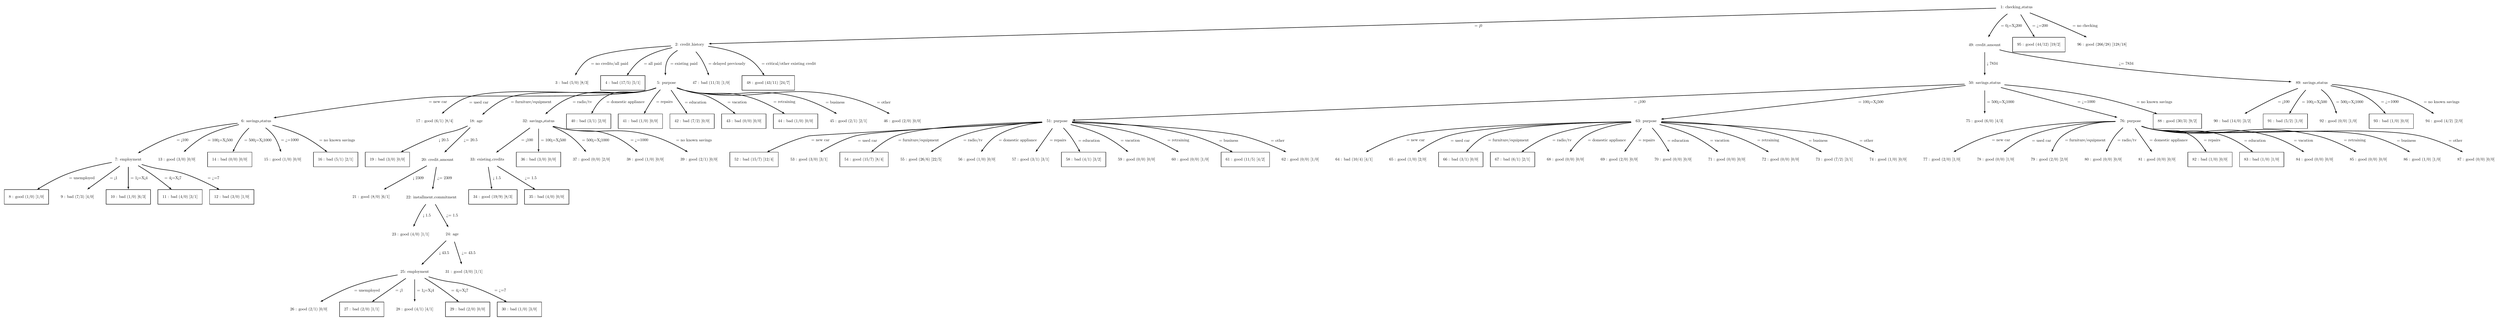
\begin{tikzpicture}[>=latex,line join=bevel,]
  \pgfsetlinewidth{1bp}
%%
\pgfsetcolor{black}
  % Edge: N6996db8 -> N76ccd017
  \draw [->,very thick] (4901.2bp,562.8bp) .. controls (4969.4bp,545.28bp) and (5108.2bp,509.61bp)  .. (5187.5bp,489.22bp);
  \definecolor{strokecol}{rgb}{0.0,0.0,0.0};
  \pgfsetstrokecolor{strokecol}
  \draw (5111.0bp,527.0bp) node { = >=1000};
  % Edge: N6504e3b2 -> N515f550a
  \draw [->,very thick] (3993.3bp,478.62bp) .. controls (3880.4bp,477.18bp) and (3542.7bp,470.71bp)  .. (3436.5bp,444.0bp) .. controls (3406.5bp,436.45bp) and (3374.8bp,421.61bp)  .. (3342.2bp,404.07bp);
  \draw (3464.5bp,433.0bp) node { = new car};
  % Edge: N3581c5f3 -> N5fcfe4b2
  \draw [->,very thick] (1599.8bp,561.72bp) .. controls (1593.9bp,559.5bp) and (1587.6bp,557.43bp)  .. (1581.5bp,556.0bp) .. controls (1498.1bp,536.37bp) and (1469.6bp,568.38bp)  .. (1389.5bp,538.0bp) .. controls (1369.4bp,530.38bp) and (1349.8bp,516.09bp)  .. (1327.9bp,497.1bp);
  \draw (1419.0bp,527.0bp) node { = radio/tv};
  % Edge: N1963006a -> N3d012ddd
  \draw [->,very thick] (2621.1bp,476.35bp) .. controls (2664.2bp,472.46bp) and (2737.4bp,463.46bp)  .. (2797.5bp,444.0bp) .. controls (2824.4bp,435.29bp) and (2852.8bp,421.08bp)  .. (2883.5bp,404.01bp);
  \draw (2882.0bp,433.0bp) node { = retraining};
  % Edge: N3581c5f3 -> N726f3b58
  \draw [->,very thick] (1651.2bp,561.79bp) .. controls (1657.1bp,559.57bp) and (1663.5bp,557.48bp)  .. (1669.5bp,556.0bp) .. controls (1740.3bp,538.72bp) and (1762.7bp,559.12bp)  .. (1832.5bp,538.0bp) .. controls (1858.9bp,530.02bp) and (1886.4bp,515.76bp)  .. (1916.1bp,498.22bp);
  \draw (1915.0bp,527.0bp) node { = retraining};
  % Edge: N76ccd017 -> N762efe5d
  \draw [->,very thick] (5246.4bp,467.58bp) .. controls (5252.5bp,465.37bp) and (5259.2bp,463.33bp)  .. (5265.5bp,462.0bp) .. controls (5394.5bp,434.86bp) and (5434.5bp,479.08bp)  .. (5561.5bp,444.0bp) .. controls (5588.5bp,436.54bp) and (5616.6bp,421.89bp)  .. (5646.1bp,404.08bp);
  \draw (5644.0bp,433.0bp) node { = vacation};
  % Edge: N4ee285c6 -> N20fa23c1
  \draw [->,very thick] (1639.7bp,660.74bp) .. controls (1616.0bp,655.76bp) and (1587.0bp,647.04bp)  .. (1564.5bp,632.0bp) .. controls (1552.4bp,623.9bp) and (1541.9bp,611.66bp)  .. (1528.3bp,592.07bp);
  \draw (1592.0bp,621.0bp) node { = all paid};
  % Edge: N1963006a -> N7dc5e7b4
  \draw [->,very thick] (2572.9bp,462.55bp) .. controls (2563.1bp,448.68bp) and (2548.9bp,428.6bp)  .. (2531.7bp,404.24bp);
  \draw (2586.5bp,433.0bp) node { = repairs};
  % Edge: N504bae78 -> N484b61fc
  \draw [->,very thick] (1007.5bp,91.647bp) .. controls (1007.5bp,78.823bp) and (1007.5bp,61.108bp)  .. (1007.5bp,36.3bp);
  \draw (1034.0bp,64.0bp) node { = 1<=X<4};
  % Edge: N4e515669 -> N17d10166
  \draw [->,very thick] (1037.3bp,370.54bp) .. controls (1011.1bp,356.09bp) and (970.54bp,333.67bp)  .. (931.35bp,312.03bp);
  \draw (1016.5bp,340.0bp) node { < 2309};
  % Edge: N3581c5f3 -> N61e717c2
  \draw [->,very thick] (1600.3bp,561.65bp) .. controls (1594.3bp,559.38bp) and (1587.8bp,557.3bp)  .. (1581.5bp,556.0bp) .. controls (1484.4bp,535.85bp) and (1229.3bp,570.39bp)  .. (1135.5bp,538.0bp) .. controls (1115.4bp,531.06bp) and (1096.0bp,517.19bp)  .. (1073.9bp,498.24bp);
  \draw (1165.0bp,527.0bp) node { = used car};
  % Edge: N6aa8ceb6 -> N1a93a7ca
  \draw [->,very thick] (600.67bp,463.21bp) .. controls (594.79bp,457.5bp) and (588.49bp,450.78bp)  .. (583.5bp,444.0bp) .. controls (576.56bp,434.58bp) and (570.29bp,423.35bp)  .. (560.91bp,404.25bp);
  \draw (622.5bp,433.0bp) node { = 500<=X<1000};
  % Edge: N4e515669 -> N1b9e1916
  \draw [->,very thick] (1060.6bp,367.65bp) .. controls (1058.5bp,354.74bp) and (1055.5bp,336.88bp)  .. (1051.3bp,311.99bp);
  \draw (1081.0bp,340.0bp) node { >= 2309};
  % Edge: N6504e3b2 -> N156643d4
  \draw [->,very thick] (4063.5bp,471.82bp) .. controls (4087.0bp,466.02bp) and (4119.1bp,456.72bp)  .. (4145.5bp,444.0bp) .. controls (4164.5bp,434.85bp) and (4184.0bp,421.67bp)  .. (4207.4bp,404.18bp);
  \draw (4211.0bp,433.0bp) node { = vacation};
  % Edge: N76ccd017 -> N53bd815b
  \draw [->,very thick] (5200.8bp,464.16bp) .. controls (5194.2bp,458.33bp) and (5187.0bp,451.29bp)  .. (5181.5bp,444.0bp) .. controls (5174.4bp,434.68bp) and (5168.3bp,423.38bp)  .. (5159.3bp,404.13bp);
  \draw (5211.0bp,433.0bp) node { = radio/tv};
  % Edge: N368102c8 -> N71dac704
  \draw [->,very thick] (4897.8bp,655.44bp) .. controls (4905.2bp,653.38bp) and (4913.1bp,651.43bp)  .. (4920.5bp,650.0bp) .. controls (5171.9bp,601.52bp) and (5477.5bp,583.23bp)  .. (5614.9bp,576.92bp);
  \draw (5209.0bp,621.0bp) node { >= 7834};
  % Edge: N5fcfe4b2 -> Nea30797
  \draw [->,very thick] (1346.0bp,466.73bp) .. controls (1359.9bp,460.95bp) and (1375.6bp,453.27bp)  .. (1388.5bp,444.0bp) .. controls (1400.9bp,435.06bp) and (1412.7bp,422.89bp)  .. (1428.6bp,404.17bp);
  \draw (1451.5bp,433.0bp) node { = 500<=X<1000};
  % Edge: N6504e3b2 -> N1175e2db
  \draw [->,very thick] (4067.4bp,477.65bp) .. controls (4161.1bp,473.97bp) and (4406.3bp,462.79bp)  .. (4485.5bp,444.0bp) .. controls (4519.1bp,436.03bp) and (4555.1bp,421.06bp)  .. (4591.2bp,404.12bp);
  \draw (4571.0bp,433.0bp) node { = other};
  % Edge: N76ccd017 -> N4926097b
  \draw [->,very thick] (5246.9bp,467.58bp) .. controls (5252.9bp,465.43bp) and (5259.4bp,463.41bp)  .. (5265.5bp,462.0bp) .. controls (5345.6bp,443.61bp) and (5371.7bp,470.32bp)  .. (5449.5bp,444.0bp) .. controls (5471.9bp,436.41bp) and (5494.6bp,422.48bp)  .. (5520.3bp,404.12bp);
  \draw (5525.0bp,433.0bp) node { = education};
  % Edge: N76ccd017 -> N3830f1c0
  \draw [->,very thick] (5246.3bp,467.42bp) .. controls (5252.5bp,465.22bp) and (5259.1bp,463.23bp)  .. (5265.5bp,462.0bp) .. controls (5410.4bp,434.04bp) and (5785.1bp,474.68bp)  .. (5929.5bp,444.0bp) .. controls (5963.5bp,436.77bp) and (5999.8bp,421.46bp)  .. (6035.7bp,404.07bp);
  \draw (6017.0bp,433.0bp) node { = other};
  % Edge: N5fcfe4b2 -> N73a8dfcc
  \draw [->,very thick] (1311.5bp,461.7bp) .. controls (1311.5bp,448.46bp) and (1311.5bp,429.95bp)  .. (1311.5bp,404.23bp);
  \draw (1348.0bp,433.0bp) node { = 100<=X<500};
  % Edge: N4f8e5cde -> N4c98385c
  \draw [->,very thick] (1105.0bp,184.07bp) .. controls (1109.1bp,171.08bp) and (1115.0bp,152.89bp)  .. (1123.0bp,128.16bp);
  \draw (1140.0bp,156.0bp) node { >= 43.5};
  % Edge: N7506e922 -> N368102c8
  \draw [->,very thick] (4917.2bp,743.63bp) .. controls (4909.8bp,737.96bp) and (4901.9bp,731.15bp)  .. (4895.5bp,724.0bp) .. controls (4887.7bp,715.22bp) and (4880.6bp,704.44bp)  .. (4870.0bp,685.9bp);
  \draw (4927.0bp,714.0bp) node { = 0<=X<200};
  % Edge: N504bae78 -> N759ebb3d
  \draw [->,very thick] (985.74bp,93.936bp) .. controls (965.27bp,79.764bp) and (934.33bp,58.341bp)  .. (902.44bp,36.269bp);
  \draw (969.5bp,64.0bp) node { = <1};
  % Edge: N7506e922 -> N6f75e721
  \draw [->,very thick] (4949.8bp,742.07bp) .. controls (4957.9bp,728.83bp) and (4969.3bp,710.19bp)  .. (4984.0bp,686.16bp);
  \draw (4997.5bp,714.0bp) node { = >=200};
  % Edge: N71dac704 -> N73a28541
  \draw [->,very thick] (5713.5bp,570.29bp) .. controls (5759.5bp,566.59bp) and (5829.7bp,557.96bp)  .. (5887.5bp,538.0bp) .. controls (5911.7bp,529.65bp) and (5936.8bp,515.71bp)  .. (5964.7bp,498.17bp);
  \draw (5983.0bp,527.0bp) node { = no known savings};
  % Edge: N5fcfe4b2 -> N3f8f9dd6
  \draw [->,very thick] (1347.4bp,467.42bp) .. controls (1355.0bp,465.33bp) and (1363.0bp,463.38bp)  .. (1370.5bp,462.0bp) .. controls (1467.0bp,444.33bp) and (1496.0bp,470.25bp)  .. (1590.5bp,444.0bp) .. controls (1618.4bp,436.24bp) and (1647.7bp,421.65bp)  .. (1678.3bp,404.16bp);
  \draw (1693.0bp,433.0bp) node { = no known savings};
  % Edge: N76ccd017 -> N4361bd48
  \draw [->,very thick] (5182.4bp,479.74bp) .. controls (5146.0bp,478.66bp) and (5090.6bp,471.95bp)  .. (5052.5bp,444.0bp) .. controls (5042.2bp,436.42bp) and (5034.7bp,424.44bp)  .. (5025.7bp,404.1bp);
  \draw (5108.5bp,433.0bp) node { = furniture/equipment};
  % Edge: N4ee285c6 -> N15615099
  \draw [->,very thick] (1697.7bp,650.66bp) .. controls (1702.5bp,645.02bp) and (1707.6bp,638.48bp)  .. (1711.5bp,632.0bp) .. controls (1717.3bp,622.5bp) and (1722.3bp,611.36bp)  .. (1729.8bp,592.09bp);
  \draw (1774.0bp,621.0bp) node { = delayed previously};
  % Edge: N6504e3b2 -> N379619aa
  \draw [->,very thick] (3993.8bp,476.74bp) .. controls (3962.1bp,473.37bp) and (3916.0bp,464.96bp)  .. (3881.5bp,444.0bp) .. controls (3868.5bp,436.12bp) and (3857.2bp,423.63bp)  .. (3842.8bp,404.05bp);
  \draw (3934.0bp,433.0bp) node { = domestic appliance};
  % Edge: N1963006a -> Nc2e1f26
  \draw [->,very thick] (2547.5bp,478.25bp) .. controls (2462.1bp,476.12bp) and (2253.7bp,468.5bp)  .. (2188.5bp,444.0bp) .. controls (2169.1bp,436.7bp) and (2150.2bp,423.14bp)  .. (2128.0bp,404.21bp);
  \draw (2244.5bp,433.0bp) node { = furniture/equipment};
  % Edge: N6504e3b2 -> Ncac736f
  \draw [->,very thick] (4018.7bp,462.55bp) .. controls (4008.8bp,448.68bp) and (3994.3bp,428.6bp)  .. (3976.9bp,404.24bp);
  \draw (4031.5bp,433.0bp) node { = repairs};
  % Edge: N504bae78 -> N45fe3ee3
  \draw [->,very thick] (1032.0bp,94.683bp) .. controls (1042.2bp,88.531bp) and (1054.0bp,81.128bp)  .. (1064.5bp,74.0bp) .. controls (1079.0bp,64.104bp) and (1094.6bp,52.478bp)  .. (1115.9bp,36.161bp);
  \draw (1118.0bp,64.0bp) node { = 4<=X<7};
  % Edge: N76ccd017 -> N41a4555e
  \draw [->,very thick] (5246.3bp,467.45bp) .. controls (5252.5bp,465.25bp) and (5259.2bp,463.25bp)  .. (5265.5bp,462.0bp) .. controls (5383.5bp,438.85bp) and (5689.2bp,470.8bp)  .. (5806.5bp,444.0bp) .. controls (5838.2bp,436.74bp) and (5871.8bp,421.64bp)  .. (5905.9bp,404.02bp);
  \draw (5896.5bp,433.0bp) node { = business};
  % Edge: N6aa8ceb6 -> N3d82c5f3
  \draw [->,very thick] (641.53bp,463.84bp) .. controls (648.67bp,458.27bp) and (656.07bp,451.48bp)  .. (661.5bp,444.0bp) .. controls (668.04bp,434.99bp) and (672.92bp,423.78bp)  .. (679.42bp,404.1bp);
  \draw (701.0bp,433.0bp) node { = >=1000};
  % Edge: N6504e3b2 -> N5e91993f
  \draw [->,very thick] (3993.4bp,478.76bp) .. controls (3908.0bp,477.71bp) and (3699.8bp,472.25bp)  .. (3636.5bp,444.0bp) .. controls (3620.4bp,436.82bp) and (3605.9bp,423.63bp)  .. (3588.5bp,404.2bp);
  \draw (3692.5bp,433.0bp) node { = furniture/equipment};
  % Edge: N6996db8 -> N39ed3c8d
  \draw [->,very thick] (4909.9bp,569.41bp) .. controls (4966.2bp,564.67bp) and (5061.8bp,554.89bp)  .. (5142.5bp,538.0bp) .. controls (5187.8bp,528.52bp) and (5237.9bp,513.49bp)  .. (5285.3bp,498.03bp);
  \draw (5278.0bp,527.0bp) node { = no known savings};
  % Edge: N2530c12 -> N48533e64
  \draw [->,very thick] (283.58bp,369.94bp) .. controls (263.98bp,355.83bp) and (234.4bp,334.53bp)  .. (203.48bp,312.27bp);
  \draw (268.5bp,340.0bp) node { = <1};
  % Edge: N71dac704 -> N2d363fb3
  \draw [->,very thick] (5649.6bp,556.7bp) .. controls (5644.6bp,550.95bp) and (5639.1bp,544.34bp)  .. (5634.5bp,538.0bp) .. controls (5627.3bp,528.16bp) and (5620.2bp,516.81bp)  .. (5609.1bp,498.16bp);
  \draw (5671.0bp,527.0bp) node { = 100<=X<500};
  % Edge: N3581c5f3 -> N58d25a40
  \draw [->,very thick] (1636.8bp,556.55bp) .. controls (1646.3bp,542.68bp) and (1660.0bp,522.6bp)  .. (1676.7bp,498.24bp);
  \draw (1697.0bp,527.0bp) node { = education};
  % Edge: N2530c12 -> N64a294a6
  \draw [->,very thick] (304.5bp,367.65bp) .. controls (304.5bp,354.82bp) and (304.5bp,337.11bp)  .. (304.5bp,312.3bp);
  \draw (331.0bp,340.0bp) node { = 1<=X<4};
  % Edge: N71dac704 -> N5aaa6d82
  \draw [->,very thick] (5710.8bp,567.16bp) .. controls (5738.2bp,562.26bp) and (5772.8bp,553.47bp)  .. (5800.5bp,538.0bp) .. controls (5815.1bp,529.81bp) and (5828.8bp,517.08bp)  .. (5846.0bp,498.17bp);
  \draw (5856.0bp,527.0bp) node { = >=1000};
  % Edge: N3581c5f3 -> N1b701da1
  \draw [->,very thick] (1651.9bp,562.34bp) .. controls (1657.6bp,560.14bp) and (1663.8bp,557.91bp)  .. (1669.5bp,556.0bp) .. controls (1697.5bp,546.67bp) and (1706.8bp,550.61bp)  .. (1733.5bp,538.0bp) .. controls (1752.6bp,529.01bp) and (1772.0bp,515.72bp)  .. (1795.1bp,498.07bp);
  \draw (1799.0bp,527.0bp) node { = vacation};
  % Edge: N3581c5f3 -> N442d9b6e
  \draw [->,very thick] (1651.2bp,561.59bp) .. controls (1657.1bp,559.38bp) and (1663.4bp,557.34bp)  .. (1669.5bp,556.0bp) .. controls (1792.2bp,529.06bp) and (1829.9bp,569.31bp)  .. (1951.5bp,538.0bp) .. controls (1981.1bp,530.38bp) and (2012.2bp,515.55bp)  .. (2044.3bp,498.03bp);
  \draw (2039.5bp,527.0bp) node { = business};
  % Edge: N1963006a -> N75a1cd57
  \draw [->,very thick] (2617.8bp,471.9bp) .. controls (2641.3bp,466.16bp) and (2673.3bp,456.9bp)  .. (2699.5bp,444.0bp) .. controls (2717.8bp,435.0bp) and (2736.4bp,421.98bp)  .. (2759.3bp,404.22bp);
  \draw (2764.0bp,433.0bp) node { = vacation};
  % Edge: N76ccd017 -> N5d22bbb7
  \draw [->,very thick] (5246.3bp,467.5bp) .. controls (5252.5bp,465.3bp) and (5259.2bp,463.28bp)  .. (5265.5bp,462.0bp) .. controls (5445.2bp,425.8bp) and (5499.2bp,486.54bp)  .. (5677.5bp,444.0bp) .. controls (5708.4bp,436.64bp) and (5740.9bp,421.69bp)  .. (5774.1bp,404.2bp);
  \draw (5770.0bp,433.0bp) node { = retraining};
  % Edge: N4f8e5cde -> N504bae78
  \draw [->,very thick] (1084.7bp,186.54bp) .. controls (1070.3bp,172.41bp) and (1048.0bp,150.66bp)  .. (1023.8bp,126.94bp);
  \draw (1080.0bp,156.0bp) node { < 43.5};
  % Edge: N6aa8ceb6 -> N2530c12
  \draw [->,very thick] (572.86bp,474.93bp) .. controls (531.5bp,470.33bp) and (469.28bp,461.15bp)  .. (417.5bp,444.0bp) .. controls (389.03bp,434.57bp) and (358.79bp,418.99bp)  .. (327.86bp,401.36bp);
  \draw (437.5bp,433.0bp) node { = <100};
  % Edge: N6aa8ceb6 -> N6ae40994
  \draw [->,very thick] (576.08bp,471.65bp) .. controls (551.09bp,466.23bp) and (519.41bp,457.43bp)  .. (493.5bp,444.0bp) .. controls (476.91bp,435.4bp) and (460.58bp,422.44bp)  .. (440.47bp,404.22bp);
  \draw (530.0bp,433.0bp) node { = 100<=X<500};
  % Edge: N5fcfe4b2 -> N6bf2d08e
  \draw [->,very thick] (1290.4bp,463.6bp) .. controls (1269.8bp,448.57bp) and (1238.3bp,425.55bp)  .. (1207.1bp,402.76bp);
  \draw (1283.5bp,433.0bp) node { = <100};
  % Edge: N6996db8 -> N1963006a
  \draw [->,very thick] (4812.1bp,571.0bp) .. controls (4511.0bp,558.84bp) and (2926.0bp,494.8bp)  .. (2621.3bp,482.49bp);
  \draw (4014.5bp,527.0bp) node { = <100};
  % Edge: N6504e3b2 -> N626b2d4a
  \draw [->,very thick] (3993.5bp,478.47bp) .. controls (3894.9bp,476.71bp) and (3628.3bp,469.67bp)  .. (3544.5bp,444.0bp) .. controls (3520.1bp,436.53bp) and (3495.2bp,422.18bp)  .. (3468.1bp,404.01bp);
  \draw (3574.0bp,433.0bp) node { = used car};
  % Edge: N4ee285c6 -> N1edf1c96
  \draw [->,very thick] (1727.9bp,663.86bp) .. controls (1758.6bp,659.98bp) and (1798.9bp,651.32bp)  .. (1829.5bp,632.0bp) .. controls (1841.9bp,624.18bp) and (1852.4bp,611.86bp)  .. (1866.0bp,592.04bp);
  \draw (1926.0bp,621.0bp) node { = critical/other existing credit};
  % Edge: N1963006a -> N1eb44e46
  \draw [->,very thick] (2621.3bp,477.6bp) .. controls (2714.7bp,473.8bp) and (2959.4bp,462.37bp)  .. (3038.5bp,444.0bp) .. controls (3073.0bp,436.0bp) and (3110.0bp,421.03bp)  .. (3147.2bp,404.1bp);
  \draw (3126.0bp,433.0bp) node { = other};
  % Edge: N71dac704 -> N7d6f77cc
  \draw [->,very thick] (5687.5bp,557.84bp) .. controls (5694.7bp,552.27bp) and (5702.1bp,545.48bp)  .. (5707.5bp,538.0bp) .. controls (5714.0bp,528.99bp) and (5718.9bp,517.78bp)  .. (5725.4bp,498.1bp);
  \draw (5757.5bp,527.0bp) node { = 500<=X<1000};
  % Edge: N4ee285c6 -> N3581c5f3
  \draw [->,very thick] (1652.8bp,653.96bp) .. controls (1643.8bp,648.5bp) and (1634.9bp,641.24bp)  .. (1629.5bp,632.0bp) .. controls (1624.4bp,623.19bp) and (1622.7bp,612.27bp)  .. (1622.9bp,592.12bp);
  \draw (1668.5bp,621.0bp) node { = existing paid};
  % Edge: N6bf2d08e -> N53e25b76
  \draw [->,very thick] (1209.9bp,369.94bp) .. controls (1233.2bp,355.59bp) and (1268.5bp,333.83bp)  .. (1303.7bp,312.11bp);
  \draw (1292.5bp,340.0bp) node { >= 1.5};
  % Edge: N3581c5f3 -> N6aa8ceb6
  \draw [->,very thick] (1600.3bp,561.62bp) .. controls (1594.3bp,559.35bp) and (1587.8bp,557.27bp)  .. (1581.5bp,556.0bp) .. controls (1462.8bp,531.82bp) and (1157.2bp,548.2bp)  .. (1036.5bp,538.0bp) .. controls (904.32bp,526.83bp) and (749.94bp,502.94bp)  .. (660.77bp,488.23bp);
  \draw (1064.5bp,527.0bp) node { = new car};
  % Edge: N6504e3b2 -> N7de26db8
  \draw [->,very thick] (4067.5bp,478.99bp) .. controls (4130.1bp,478.12bp) and (4260.6bp,472.65bp)  .. (4366.5bp,444.0bp) .. controls (4396.8bp,435.8bp) and (4429.0bp,421.1bp)  .. (4462.2bp,404.05bp);
  \draw (4452.5bp,433.0bp) node { = business};
  % Edge: N5fcfe4b2 -> N7e774085
  \draw [->,very thick] (1348.1bp,467.61bp) .. controls (1355.5bp,465.56bp) and (1363.2bp,463.57bp)  .. (1370.5bp,462.0bp) .. controls (1424.9bp,450.26bp) and (1442.9bp,464.89bp)  .. (1494.5bp,444.0bp) .. controls (1513.8bp,436.2bp) and (1532.7bp,422.76bp)  .. (1555.3bp,404.13bp);
  \draw (1559.0bp,433.0bp) node { = >=1000};
  % Edge: N1963006a -> N6f2b958e
  \draw [->,very thick] (2621.5bp,478.89bp) .. controls (2683.9bp,477.86bp) and (2813.3bp,472.17bp)  .. (2918.5bp,444.0bp) .. controls (2949.2bp,435.77bp) and (2982.0bp,421.07bp)  .. (3015.7bp,404.04bp);
  \draw (3005.5bp,433.0bp) node { = business};
  % Edge: N76ccd017 -> N182decdb
  \draw [->,very thick] (5182.3bp,479.48bp) .. controls (5118.1bp,479.37bp) and (4982.7bp,475.05bp)  .. (4873.5bp,444.0bp) .. controls (4845.4bp,436.01bp) and (4815.9bp,421.57bp)  .. (4784.7bp,404.26bp);
  \draw (4901.5bp,433.0bp) node { = new car};
  % Edge: N1963006a -> N1ee0005
  \draw [->,very thick] (2599.9bp,463.59bp) .. controls (2605.4bp,457.7bp) and (2611.5bp,450.77bp)  .. (2616.5bp,444.0bp) .. controls (2623.6bp,434.36bp) and (2630.4bp,423.08bp)  .. (2640.9bp,404.06bp);
  \draw (2663.0bp,433.0bp) node { = education};
  % Edge: N6996db8 -> N6504e3b2
  \draw [->,very thick] (4814.4bp,567.79bp) .. controls (4668.1bp,551.58bp) and (4221.9bp,502.19bp)  .. (4066.4bp,484.97bp);
  \draw (4582.0bp,527.0bp) node { = 100<=X<500};
  % Edge: N504bae78 -> N4cdf35a9
  \draw [->,very thick] (1041.7bp,97.892bp) .. controls (1048.5bp,95.816bp) and (1055.7bp,93.752bp)  .. (1062.5bp,92.0bp) .. controls (1100.3bp,82.223bp) and (1111.5bp,86.452bp)  .. (1148.5bp,74.0bp) .. controls (1174.7bp,65.17bp) and (1202.8bp,51.955bp)  .. (1233.8bp,36.003bp);
  \draw (1217.5bp,64.0bp) node { = >=7};
  % Edge: N66cd51c3 -> N4dcbadb4
  \draw [->,very thick] (1137.4bp,468.38bp) .. controls (1132.6bp,466.13bp) and (1127.4bp,463.87bp)  .. (1122.5bp,462.0bp) .. controls (1096.1bp,451.94bp) and (1087.9bp,454.05bp)  .. (1061.5bp,444.0bp) .. controls (1034.6bp,433.77bp) and (1005.4bp,420.08bp)  .. (973.29bp,404.12bp);
  \draw (1079.0bp,433.0bp) node { < 20.5};
  % Edge: N7506e922 -> N4ee285c6
  \draw [->,very thick] (4889.3bp,757.61bp) .. controls (4513.0bp,747.22bp) and (2136.9bp,681.56bp)  .. (1728.9bp,670.28bp);
  \draw (3618.5bp,714.0bp) node { = <0};
  % Edge: N3581c5f3 -> Naec6354
  \draw [->,very thick] (1599.3bp,561.86bp) .. controls (1593.5bp,559.69bp) and (1587.3bp,557.59bp)  .. (1581.5bp,556.0bp) .. controls (1534.1bp,543.08bp) and (1513.8bp,564.63bp)  .. (1472.5bp,538.0bp) .. controls (1461.0bp,530.59bp) and (1452.2bp,518.36bp)  .. (1441.3bp,498.04bp);
  \draw (1525.0bp,527.0bp) node { = domestic appliance};
  % Edge: N6504e3b2 -> N1c4af82c
  \draw [->,very thick] (3993.4bp,478.12bp) .. controls (3945.9bp,475.96bp) and (3861.8bp,468.64bp)  .. (3794.5bp,444.0bp) .. controls (3772.4bp,435.91bp) and (3749.9bp,422.11bp)  .. (3724.2bp,404.04bp);
  \draw (3824.0bp,433.0bp) node { = radio/tv};
  % Edge: N3581c5f3 -> N1c655221
  \draw [->,very thick] (1610.6bp,557.53bp) .. controls (1605.2bp,551.64bp) and (1599.3bp,544.72bp)  .. (1594.5bp,538.0bp) .. controls (1587.5bp,528.3bp) and (1580.7bp,517.01bp)  .. (1570.2bp,498.01bp);
  \draw (1620.5bp,527.0bp) node { = repairs};
  % Edge: N3581c5f3 -> N66cd51c3
  \draw [->,very thick] (1599.9bp,561.53bp) .. controls (1593.9bp,559.33bp) and (1587.6bp,557.3bp)  .. (1581.5bp,556.0bp) .. controls (1506.6bp,540.01bp) and (1309.7bp,563.43bp)  .. (1237.5bp,538.0bp) .. controls (1216.1bp,530.46bp) and (1195.4bp,515.17bp)  .. (1173.0bp,495.5bp);
  \draw (1293.5bp,527.0bp) node { = furniture/equipment};
  % Edge: N1963006a -> N6d9c638
  \draw [->,very thick] (2548.1bp,476.86bp) .. controls (2516.3bp,473.57bp) and (2470.0bp,465.21bp)  .. (2435.5bp,444.0bp) .. controls (2422.7bp,436.12bp) and (2411.6bp,423.63bp)  .. (2397.6bp,404.05bp);
  \draw (2488.0bp,433.0bp) node { = domestic appliance};
  % Edge: N1963006a -> Ndcf3e99
  \draw [->,very thick] (2547.5bp,477.82bp) .. controls (2500.1bp,475.35bp) and (2416.1bp,467.7bp)  .. (2348.5bp,444.0bp) .. controls (2325.2bp,435.83bp) and (2301.2bp,421.98bp)  .. (2274.2bp,404.26bp);
  \draw (2378.0bp,433.0bp) node { = radio/tv};
  % Edge: N2530c12 -> N3b95a09c
  \draw [->,very thick] (337.42bp,373.84bp) .. controls (344.03bp,371.77bp) and (350.96bp,369.72bp)  .. (357.5bp,368.0bp) .. controls (395.69bp,357.96bp) and (407.1bp,362.67bp)  .. (444.5bp,350.0bp) .. controls (470.36bp,341.24bp) and (497.97bp,328.02bp)  .. (528.4bp,312.05bp);
  \draw (513.5bp,340.0bp) node { = >=7};
  % Edge: N76ccd017 -> N26f0a63f
  \draw [->,very thick] (5182.5bp,479.0bp) .. controls (5132.8bp,477.85bp) and (5042.6bp,471.67bp)  .. (4971.5bp,444.0bp) .. controls (4951.3bp,436.14bp) and (4931.2bp,422.52bp)  .. (4907.8bp,404.13bp);
  \draw (5001.0bp,433.0bp) node { = used car};
  % Edge: N1b9e1916 -> Nba8a1dc
  \draw [->,very thick] (1034.8bp,276.05bp) .. controls (1030.6bp,270.48bp) and (1026.1bp,264.13bp)  .. (1022.5bp,258.0bp) .. controls (1017.3bp,249.11bp) and (1012.4bp,238.93bp)  .. (1004.3bp,220.32bp);
  \draw (1037.5bp,248.0bp) node { < 1.5};
  % Edge: N7506e922 -> N69222c14
  \draw [->,very thick] (4972.3bp,746.16bp) .. controls (4988.6bp,739.67bp) and (5008.7bp,731.57bp)  .. (5026.5bp,724.0bp) .. controls (5052.0bp,713.19bp) and (5080.1bp,700.64bp)  .. (5112.3bp,686.1bp);
  \draw (5108.0bp,714.0bp) node { = no checking};
  % Edge: N1b9e1916 -> N4f8e5cde
  \draw [->,very thick] (1058.1bp,276.07bp) .. controls (1065.7bp,262.58bp) and (1076.6bp,243.48bp)  .. (1090.3bp,219.25bp);
  \draw (1099.5bp,248.0bp) node { >= 1.5};
  % Edge: N3581c5f3 -> Nee7d9f1
  \draw [->,very thick] (1650.7bp,561.67bp) .. controls (1656.7bp,559.4bp) and (1663.2bp,557.31bp)  .. (1669.5bp,556.0bp) .. controls (1845.0bp,519.21bp) and (1897.8bp,578.2bp)  .. (2072.5bp,538.0bp) .. controls (2104.9bp,530.55bp) and (2139.3bp,515.43bp)  .. (2173.9bp,498.04bp);
  \draw (2159.0bp,527.0bp) node { = other};
  % Edge: N6504e3b2 -> N5e265ba4
  \draw [->,very thick] (4045.3bp,463.46bp) .. controls (4050.6bp,457.56bp) and (4056.6bp,450.65bp)  .. (4061.5bp,444.0bp) .. controls (4068.8bp,434.21bp) and (4075.9bp,422.88bp)  .. (4087.0bp,404.21bp);
  \draw (4109.0bp,433.0bp) node { = education};
  % Edge: N6996db8 -> N36aa7bc2
  \draw [->,very thick] (4861.5bp,555.7bp) .. controls (4861.5bp,542.46bp) and (4861.5bp,523.95bp)  .. (4861.5bp,498.23bp);
  \draw (4900.5bp,527.0bp) node { = 500<=X<1000};
  % Edge: N6bf2d08e -> N5eb5c224
  \draw [->,very thick] (1188.2bp,367.65bp) .. controls (1190.2bp,354.82bp) and (1192.9bp,337.11bp)  .. (1196.8bp,312.3bp);
  \draw (1209.5bp,340.0bp) node { < 1.5};
  % Edge: N6504e3b2 -> N123a439b
  \draw [->,very thick] (4066.9bp,476.33bp) .. controls (4110.0bp,472.42bp) and (4183.9bp,463.37bp)  .. (4244.5bp,444.0bp) .. controls (4271.9bp,435.23bp) and (4301.0bp,420.93bp)  .. (4331.9bp,404.0bp);
  \draw (4330.0bp,433.0bp) node { = retraining};
  % Edge: N6aa8ceb6 -> N2b05039f
  \draw [->,very thick] (658.45bp,470.04bp) .. controls (680.87bp,464.2bp) and (708.98bp,455.52bp)  .. (732.5bp,444.0bp) .. controls (750.96bp,434.96bp) and (769.84bp,421.93bp)  .. (792.99bp,404.19bp);
  \draw (817.0bp,433.0bp) node { = no known savings};
  % Edge: N2530c12 -> N7e0b37bc
  \draw [->,very thick] (328.74bp,370.96bp) .. controls (339.02bp,364.79bp) and (351.02bp,357.3bp)  .. (361.5bp,350.0bp) .. controls (375.65bp,340.15bp) and (390.76bp,328.44bp)  .. (411.15bp,312.01bp);
  \draw (414.0bp,340.0bp) node { = 4<=X<7};
  % Edge: N1963006a -> N7fbe847c
  \draw [->,very thick] (2547.8bp,476.97bp) .. controls (2417.2bp,469.75bp) and (1982.5bp,445.63bp)  .. (1975.5bp,444.0bp) .. controls (1942.6bp,436.35bp) and (1907.5bp,421.32bp)  .. (1872.2bp,404.05bp);
  \draw (2003.5bp,433.0bp) node { = new car};
  % Edge: N1963006a -> N41975e01
  \draw [->,very thick] (2547.7bp,477.23bp) .. controls (2440.5bp,471.96bp) and (2133.3bp,455.98bp)  .. (2089.5bp,444.0bp) .. controls (2061.9bp,436.44bp) and (2033.0bp,421.94bp)  .. (2002.4bp,404.26bp);
  \draw (2119.0bp,433.0bp) node { = used car};
  % Edge: N4ee285c6 -> N621be5d1
  \draw [->,very thick] (1636.7bp,664.81bp) .. controls (1574.6bp,661.12bp) and (1467.6bp,652.02bp)  .. (1434.5bp,632.0bp) .. controls (1422.4bp,624.69bp) and (1412.8bp,612.3bp)  .. (1401.1bp,592.16bp);
  \draw (1486.0bp,621.0bp) node { = no credits/all paid};
  % Edge: N504bae78 -> N3b764bce
  \draw [->,very thick] (965.49bp,102.44bp) .. controls (934.05bp,96.824bp) and (890.32bp,87.483bp)  .. (853.5bp,74.0bp) .. controls (829.7bp,65.282bp) and (804.45bp,52.345bp)  .. (775.84bp,36.239bp);
  \draw (890.5bp,64.0bp) node { = unemployed};
  % Edge: N66cd51c3 -> N4e515669
  \draw [->,very thick] (1143.7bp,464.62bp) .. controls (1128.7bp,450.16bp) and (1105.4bp,427.62bp)  .. (1080.2bp,403.13bp);
  \draw (1145.0bp,433.0bp) node { >= 20.5};
  % Edge: N2530c12 -> N73c6c3b2
  \draw [->,very thick] (263.85bp,378.76bp) .. controls (232.92bp,373.25bp) and (189.66bp,363.92bp)  .. (153.5bp,350.0bp) .. controls (131.11bp,341.38bp) and (107.57bp,328.48bp)  .. (80.41bp,312.04bp);
  \draw (190.5bp,340.0bp) node { = unemployed};
  % Edge: N368102c8 -> N6996db8
  \draw [->,very thick] (4861.5bp,649.7bp) .. controls (4861.5bp,636.46bp) and (4861.5bp,617.95bp)  .. (4861.5bp,592.23bp);
  \draw (4880.5bp,621.0bp) node { < 7834};
  % Edge: N76ccd017 -> N2401f4c3
  \draw [->,very thick] (5231.1bp,462.55bp) .. controls (5240.9bp,448.68bp) and (5255.1bp,428.6bp)  .. (5272.3bp,404.24bp);
  \draw (5313.0bp,433.0bp) node { = domestic appliance};
  % Edge: N76ccd017 -> N7637f22
  \draw [->,very thick] (5247.0bp,467.92bp) .. controls (5253.0bp,465.75bp) and (5259.4bp,463.64bp)  .. (5265.5bp,462.0bp) .. controls (5310.8bp,449.82bp) and (5329.2bp,467.99bp)  .. (5369.5bp,444.0bp) .. controls (5382.1bp,436.52bp) and (5392.5bp,424.12bp)  .. (5405.6bp,404.04bp);
  \draw (5419.5bp,433.0bp) node { = repairs};
  % Edge: N71dac704 -> N123772c4
  \draw [->,very thick] (5630.3bp,560.64bp) .. controls (5613.6bp,554.32bp) and (5593.3bp,546.24bp)  .. (5575.5bp,538.0bp) .. controls (5552.6bp,527.41bp) and (5527.8bp,514.15bp)  .. (5499.2bp,498.18bp);
  \draw (5595.5bp,527.0bp) node { = <100};
  % Node: N484b61fc
\begin{scope}
  \definecolor{strokecol}{rgb}{0.0,0.0,0.0};
  \pgfsetstrokecolor{strokecol}
  \draw (1007.5bp,18.0bp) node {28 : good (4/1) [4/1]};
\end{scope}
  % Node: N6aa8ceb6
\begin{scope}
  \definecolor{strokecol}{rgb}{0.0,0.0,0.0};
  \pgfsetstrokecolor{strokecol}
  \draw (618.5bp,480.0bp) node {6: savings\_status};
\end{scope}
  % Node: N6504e3b2
\begin{scope}
  \definecolor{strokecol}{rgb}{0.0,0.0,0.0};
  \pgfsetstrokecolor{strokecol}
  \draw (4030.5bp,480.0bp) node {63: purpose};
\end{scope}
  % Node: N41a4555e
\begin{scope}
  \definecolor{strokecol}{rgb}{0.0,0.0,0.0};
  \pgfsetstrokecolor{strokecol}
  \draw (5935.5bp,386.0bp) node {86 : good (1/0) [1/0]};
\end{scope}
  % Node: N5e91993f
\begin{scope}
  \definecolor{strokecol}{rgb}{0.0,0.0,0.0};
  \pgfsetstrokecolor{strokecol}
  \draw (3630.0bp,404.0bp) -- (3521.0bp,404.0bp) -- (3521.0bp,368.0bp) -- (3630.0bp,368.0bp) -- cycle;
  \draw (3575.5bp,386.0bp) node {66 : bad (3/1) [0/0]};
\end{scope}
  % Node: N53bd815b
\begin{scope}
  \definecolor{strokecol}{rgb}{0.0,0.0,0.0};
  \pgfsetstrokecolor{strokecol}
  \draw (5152.5bp,386.0bp) node {80 : good (0/0) [0/0]};
\end{scope}
  % Node: N4e515669
\begin{scope}
  \definecolor{strokecol}{rgb}{0.0,0.0,0.0};
  \pgfsetstrokecolor{strokecol}
  \draw (1063.5bp,386.0bp) node {20: credit\_amount};
\end{scope}
  % Node: N442d9b6e
\begin{scope}
  \definecolor{strokecol}{rgb}{0.0,0.0,0.0};
  \pgfsetstrokecolor{strokecol}
  \draw (2072.5bp,480.0bp) node {45 : good (2/1) [2/1]};
\end{scope}
  % Node: N73a8dfcc
\begin{scope}
  \definecolor{strokecol}{rgb}{0.0,0.0,0.0};
  \pgfsetstrokecolor{strokecol}
  \draw (1366.0bp,404.0bp) -- (1257.0bp,404.0bp) -- (1257.0bp,368.0bp) -- (1366.0bp,368.0bp) -- cycle;
  \draw (1311.5bp,386.0bp) node {36 : bad (3/0) [0/0]};
\end{scope}
  % Node: N726f3b58
\begin{scope}
  \definecolor{strokecol}{rgb}{0.0,0.0,0.0};
  \pgfsetstrokecolor{strokecol}
  \draw (1997.0bp,498.0bp) -- (1888.0bp,498.0bp) -- (1888.0bp,462.0bp) -- (1997.0bp,462.0bp) -- cycle;
  \draw (1942.5bp,480.0bp) node {44 : bad (1/0) [0/0]};
\end{scope}
  % Node: N1963006a
\begin{scope}
  \definecolor{strokecol}{rgb}{0.0,0.0,0.0};
  \pgfsetstrokecolor{strokecol}
  \draw (2584.5bp,480.0bp) node {51: purpose};
\end{scope}
  % Node: N73a28541
\begin{scope}
  \definecolor{strokecol}{rgb}{0.0,0.0,0.0};
  \pgfsetstrokecolor{strokecol}
  \draw (5989.5bp,480.0bp) node {94 : good (4/2) [2/0]};
\end{scope}
  % Node: N4926097b
\begin{scope}
  \definecolor{strokecol}{rgb}{0.0,0.0,0.0};
  \pgfsetstrokecolor{strokecol}
  \draw (5596.0bp,404.0bp) -- (5487.0bp,404.0bp) -- (5487.0bp,368.0bp) -- (5596.0bp,368.0bp) -- cycle;
  \draw (5541.5bp,386.0bp) node {83 : bad (1/0) [1/0]};
\end{scope}
  % Node: N2401f4c3
\begin{scope}
  \definecolor{strokecol}{rgb}{0.0,0.0,0.0};
  \pgfsetstrokecolor{strokecol}
  \draw (5284.5bp,386.0bp) node {81 : good (0/0) [0/0]};
\end{scope}
  % Node: N4361bd48
\begin{scope}
  \definecolor{strokecol}{rgb}{0.0,0.0,0.0};
  \pgfsetstrokecolor{strokecol}
  \draw (5020.5bp,386.0bp) node {79 : good (2/0) [2/0]};
\end{scope}
  % Node: N71dac704
\begin{scope}
  \definecolor{strokecol}{rgb}{0.0,0.0,0.0};
  \pgfsetstrokecolor{strokecol}
  \draw (5664.5bp,574.0bp) node {89: savings\_status};
\end{scope}
  % Node: N2d363fb3
\begin{scope}
  \definecolor{strokecol}{rgb}{0.0,0.0,0.0};
  \pgfsetstrokecolor{strokecol}
  \draw (5654.0bp,498.0bp) -- (5545.0bp,498.0bp) -- (5545.0bp,462.0bp) -- (5654.0bp,462.0bp) -- cycle;
  \draw (5599.5bp,480.0bp) node {91 : bad (5/2) [1/0]};
\end{scope}
  % Node: N3f8f9dd6
\begin{scope}
  \definecolor{strokecol}{rgb}{0.0,0.0,0.0};
  \pgfsetstrokecolor{strokecol}
  \draw (1705.5bp,386.0bp) node {39 : good (2/1) [0/0]};
\end{scope}
  % Node: N39ed3c8d
\begin{scope}
  \definecolor{strokecol}{rgb}{0.0,0.0,0.0};
  \pgfsetstrokecolor{strokecol}
  \draw (5394.0bp,498.0bp) -- (5275.0bp,498.0bp) -- (5275.0bp,462.0bp) -- (5394.0bp,462.0bp) -- cycle;
  \draw (5334.5bp,480.0bp) node {88 : good (30/3) [9/2]};
\end{scope}
  % Node: N5aaa6d82
\begin{scope}
  \definecolor{strokecol}{rgb}{0.0,0.0,0.0};
  \pgfsetstrokecolor{strokecol}
  \draw (5914.0bp,498.0bp) -- (5805.0bp,498.0bp) -- (5805.0bp,462.0bp) -- (5914.0bp,462.0bp) -- cycle;
  \draw (5859.5bp,480.0bp) node {93 : bad (1/0) [0/0]};
\end{scope}
  % Node: N7506e922
\begin{scope}
  \definecolor{strokecol}{rgb}{0.0,0.0,0.0};
  \pgfsetstrokecolor{strokecol}
  \draw (4939.5bp,760.0bp) node {1: checking\_status};
\end{scope}
  % Node: N379619aa
\begin{scope}
  \definecolor{strokecol}{rgb}{0.0,0.0,0.0};
  \pgfsetstrokecolor{strokecol}
  \draw (3832.5bp,386.0bp) node {68 : good (0/0) [0/0]};
\end{scope}
  % Node: N182decdb
\begin{scope}
  \definecolor{strokecol}{rgb}{0.0,0.0,0.0};
  \pgfsetstrokecolor{strokecol}
  \draw (4756.5bp,386.0bp) node {77 : good (2/0) [1/0]};
\end{scope}
  % Node: N66cd51c3
\begin{scope}
  \definecolor{strokecol}{rgb}{0.0,0.0,0.0};
  \pgfsetstrokecolor{strokecol}
  \draw (1158.5bp,480.0bp) node {18: age};
\end{scope}
  % Node: N17d10166
\begin{scope}
  \definecolor{strokecol}{rgb}{0.0,0.0,0.0};
  \pgfsetstrokecolor{strokecol}
  \draw (900.5bp,294.0bp) node {21 : good (8/0) [6/1]};
\end{scope}
  % Node: N5eb5c224
\begin{scope}
  \definecolor{strokecol}{rgb}{0.0,0.0,0.0};
  \pgfsetstrokecolor{strokecol}
  \draw (1259.0bp,312.0bp) -- (1140.0bp,312.0bp) -- (1140.0bp,276.0bp) -- (1259.0bp,276.0bp) -- cycle;
  \draw (1199.5bp,294.0bp) node {34 : good (19/9) [8/3]};
\end{scope}
  % Node: N20fa23c1
\begin{scope}
  \definecolor{strokecol}{rgb}{0.0,0.0,0.0};
  \pgfsetstrokecolor{strokecol}
  \draw (1573.0bp,592.0bp) -- (1464.0bp,592.0bp) -- (1464.0bp,556.0bp) -- (1573.0bp,556.0bp) -- cycle;
  \draw (1518.5bp,574.0bp) node {4 : bad (17/5) [5/1]};
\end{scope}
  % Node: N626b2d4a
\begin{scope}
  \definecolor{strokecol}{rgb}{0.0,0.0,0.0};
  \pgfsetstrokecolor{strokecol}
  \draw (3445.5bp,386.0bp) node {65 : good (1/0) [2/0]};
\end{scope}
  % Node: Nee7d9f1
\begin{scope}
  \definecolor{strokecol}{rgb}{0.0,0.0,0.0};
  \pgfsetstrokecolor{strokecol}
  \draw (2204.5bp,480.0bp) node {46 : good (2/0) [0/0]};
\end{scope}
  % Node: N1c655221
\begin{scope}
  \definecolor{strokecol}{rgb}{0.0,0.0,0.0};
  \pgfsetstrokecolor{strokecol}
  \draw (1616.0bp,498.0bp) -- (1507.0bp,498.0bp) -- (1507.0bp,462.0bp) -- (1616.0bp,462.0bp) -- cycle;
  \draw (1561.5bp,480.0bp) node {41 : bad (1/0) [0/0]};
\end{scope}
  % Node: Naec6354
\begin{scope}
  \definecolor{strokecol}{rgb}{0.0,0.0,0.0};
  \pgfsetstrokecolor{strokecol}
  \draw (1489.0bp,498.0bp) -- (1380.0bp,498.0bp) -- (1380.0bp,462.0bp) -- (1489.0bp,462.0bp) -- cycle;
  \draw (1434.5bp,480.0bp) node {40 : bad (3/1) [2/0]};
\end{scope}
  % Node: Nc2e1f26
\begin{scope}
  \definecolor{strokecol}{rgb}{0.0,0.0,0.0};
  \pgfsetstrokecolor{strokecol}
  \draw (2170.0bp,404.0bp) -- (2051.0bp,404.0bp) -- (2051.0bp,368.0bp) -- (2170.0bp,368.0bp) -- cycle;
  \draw (2110.5bp,386.0bp) node {54 : good (15/7) [8/4]};
\end{scope}
  % Node: N4c98385c
\begin{scope}
  \definecolor{strokecol}{rgb}{0.0,0.0,0.0};
  \pgfsetstrokecolor{strokecol}
  \draw (1128.5bp,110.0bp) node {31 : good (3/0) [1/1]};
\end{scope}
  % Node: N4ee285c6
\begin{scope}
  \definecolor{strokecol}{rgb}{0.0,0.0,0.0};
  \pgfsetstrokecolor{strokecol}
  \draw (1682.5bp,668.0bp) node {2: credit\_history};
\end{scope}
  % Node: N1ee0005
\begin{scope}
  \definecolor{strokecol}{rgb}{0.0,0.0,0.0};
  \pgfsetstrokecolor{strokecol}
  \draw (2704.0bp,404.0bp) -- (2595.0bp,404.0bp) -- (2595.0bp,368.0bp) -- (2704.0bp,368.0bp) -- cycle;
  \draw (2649.5bp,386.0bp) node {58 : bad (4/1) [3/2]};
\end{scope}
  % Node: N58d25a40
\begin{scope}
  \definecolor{strokecol}{rgb}{0.0,0.0,0.0};
  \pgfsetstrokecolor{strokecol}
  \draw (1743.0bp,498.0bp) -- (1634.0bp,498.0bp) -- (1634.0bp,462.0bp) -- (1743.0bp,462.0bp) -- cycle;
  \draw (1688.5bp,480.0bp) node {42 : bad (7/2) [0/0]};
\end{scope}
  % Node: N41975e01
\begin{scope}
  \definecolor{strokecol}{rgb}{0.0,0.0,0.0};
  \pgfsetstrokecolor{strokecol}
  \draw (1975.5bp,386.0bp) node {53 : good (3/0) [3/1]};
\end{scope}
  % Node: N123772c4
\begin{scope}
  \definecolor{strokecol}{rgb}{0.0,0.0,0.0};
  \pgfsetstrokecolor{strokecol}
  \draw (5469.5bp,480.0bp) node {90 : bad (14/0) [3/2]};
\end{scope}
  % Node: Ncac736f
\begin{scope}
  \definecolor{strokecol}{rgb}{0.0,0.0,0.0};
  \pgfsetstrokecolor{strokecol}
  \draw (3964.5bp,386.0bp) node {69 : good (2/0) [0/0]};
\end{scope}
  % Node: N36aa7bc2
\begin{scope}
  \definecolor{strokecol}{rgb}{0.0,0.0,0.0};
  \pgfsetstrokecolor{strokecol}
  \draw (4861.5bp,480.0bp) node {75 : good (6/0) [4/3]};
\end{scope}
  % Node: N7de26db8
\begin{scope}
  \definecolor{strokecol}{rgb}{0.0,0.0,0.0};
  \pgfsetstrokecolor{strokecol}
  \draw (4492.5bp,386.0bp) node {73 : good (7/2) [3/1]};
\end{scope}
  % Node: N7e774085
\begin{scope}
  \definecolor{strokecol}{rgb}{0.0,0.0,0.0};
  \pgfsetstrokecolor{strokecol}
  \draw (1573.5bp,386.0bp) node {38 : good (1/0) [0/0]};
\end{scope}
  % Node: N3d82c5f3
\begin{scope}
  \definecolor{strokecol}{rgb}{0.0,0.0,0.0};
  \pgfsetstrokecolor{strokecol}
  \draw (683.5bp,386.0bp) node {15 : good (1/0) [0/0]};
\end{scope}
  % Node: N5e265ba4
\begin{scope}
  \definecolor{strokecol}{rgb}{0.0,0.0,0.0};
  \pgfsetstrokecolor{strokecol}
  \draw (4096.5bp,386.0bp) node {70 : good (0/0) [0/0]};
\end{scope}
  % Node: N1a93a7ca
\begin{scope}
  \definecolor{strokecol}{rgb}{0.0,0.0,0.0};
  \pgfsetstrokecolor{strokecol}
  \draw (608.0bp,404.0bp) -- (499.0bp,404.0bp) -- (499.0bp,368.0bp) -- (608.0bp,368.0bp) -- cycle;
  \draw (553.5bp,386.0bp) node {14 : bad (0/0) [0/0]};
\end{scope}
  % Node: N156643d4
\begin{scope}
  \definecolor{strokecol}{rgb}{0.0,0.0,0.0};
  \pgfsetstrokecolor{strokecol}
  \draw (4228.5bp,386.0bp) node {71 : good (0/0) [0/0]};
\end{scope}
  % Node: N6996db8
\begin{scope}
  \definecolor{strokecol}{rgb}{0.0,0.0,0.0};
  \pgfsetstrokecolor{strokecol}
  \draw (4861.5bp,574.0bp) node {50: savings\_status};
\end{scope}
  % Node: N4f8e5cde
\begin{scope}
  \definecolor{strokecol}{rgb}{0.0,0.0,0.0};
  \pgfsetstrokecolor{strokecol}
  \draw (1099.5bp,202.0bp) node {24: age};
\end{scope}
  % Node: N368102c8
\begin{scope}
  \definecolor{strokecol}{rgb}{0.0,0.0,0.0};
  \pgfsetstrokecolor{strokecol}
  \draw (4861.5bp,668.0bp) node {49: credit\_amount};
\end{scope}
  % Node: N7fbe847c
\begin{scope}
  \definecolor{strokecol}{rgb}{0.0,0.0,0.0};
  \pgfsetstrokecolor{strokecol}
  \draw (1900.0bp,404.0bp) -- (1781.0bp,404.0bp) -- (1781.0bp,368.0bp) -- (1900.0bp,368.0bp) -- cycle;
  \draw (1840.5bp,386.0bp) node {52 : bad (15/7) [12/4]};
\end{scope}
  % Node: N5d22bbb7
\begin{scope}
  \definecolor{strokecol}{rgb}{0.0,0.0,0.0};
  \pgfsetstrokecolor{strokecol}
  \draw (5803.5bp,386.0bp) node {85 : good (0/0) [0/0]};
\end{scope}
  % Node: N1b701da1
\begin{scope}
  \definecolor{strokecol}{rgb}{0.0,0.0,0.0};
  \pgfsetstrokecolor{strokecol}
  \draw (1870.0bp,498.0bp) -- (1761.0bp,498.0bp) -- (1761.0bp,462.0bp) -- (1870.0bp,462.0bp) -- cycle;
  \draw (1815.5bp,480.0bp) node {43 : bad (0/0) [0/0]};
\end{scope}
  % Node: N504bae78
\begin{scope}
  \definecolor{strokecol}{rgb}{0.0,0.0,0.0};
  \pgfsetstrokecolor{strokecol}
  \draw (1007.5bp,110.0bp) node {25: employment};
\end{scope}
  % Node: N1edf1c96
\begin{scope}
  \definecolor{strokecol}{rgb}{0.0,0.0,0.0};
  \pgfsetstrokecolor{strokecol}
  \draw (1940.0bp,592.0bp) -- (1811.0bp,592.0bp) -- (1811.0bp,556.0bp) -- (1940.0bp,556.0bp) -- cycle;
  \draw (1875.5bp,574.0bp) node {48 : good (43/11) [24/7]};
\end{scope}
  % Node: N69222c14
\begin{scope}
  \definecolor{strokecol}{rgb}{0.0,0.0,0.0};
  \pgfsetstrokecolor{strokecol}
  \draw (5149.5bp,668.0bp) node {96 : good (266/28) [128/18]};
\end{scope}
  % Node: N15615099
\begin{scope}
  \definecolor{strokecol}{rgb}{0.0,0.0,0.0};
  \pgfsetstrokecolor{strokecol}
  \draw (1735.5bp,574.0bp) node {47 : bad (11/3) [1/0]};
\end{scope}
  % Node: N6f2b958e
\begin{scope}
  \definecolor{strokecol}{rgb}{0.0,0.0,0.0};
  \pgfsetstrokecolor{strokecol}
  \draw (3106.0bp,404.0bp) -- (2987.0bp,404.0bp) -- (2987.0bp,368.0bp) -- (3106.0bp,368.0bp) -- cycle;
  \draw (3046.5bp,386.0bp) node {61 : good (11/5) [4/2]};
\end{scope}
  % Node: N7d6f77cc
\begin{scope}
  \definecolor{strokecol}{rgb}{0.0,0.0,0.0};
  \pgfsetstrokecolor{strokecol}
  \draw (5729.5bp,480.0bp) node {92 : good (0/0) [1/0]};
\end{scope}
  % Node: N3b764bce
\begin{scope}
  \definecolor{strokecol}{rgb}{0.0,0.0,0.0};
  \pgfsetstrokecolor{strokecol}
  \draw (747.5bp,18.0bp) node {26 : good (2/1) [0/0]};
\end{scope}
  % Node: N64a294a6
\begin{scope}
  \definecolor{strokecol}{rgb}{0.0,0.0,0.0};
  \pgfsetstrokecolor{strokecol}
  \draw (359.0bp,312.0bp) -- (250.0bp,312.0bp) -- (250.0bp,276.0bp) -- (359.0bp,276.0bp) -- cycle;
  \draw (304.5bp,294.0bp) node {10 : bad (1/0) [6/3]};
\end{scope}
  % Node: Nba8a1dc
\begin{scope}
  \definecolor{strokecol}{rgb}{0.0,0.0,0.0};
  \pgfsetstrokecolor{strokecol}
  \draw (997.5bp,202.0bp) node {23 : good (4/0) [1/1]};
\end{scope}
  % Node: N4cdf35a9
\begin{scope}
  \definecolor{strokecol}{rgb}{0.0,0.0,0.0};
  \pgfsetstrokecolor{strokecol}
  \draw (1319.0bp,36.0bp) -- (1210.0bp,36.0bp) -- (1210.0bp,0.0bp) -- (1319.0bp,0.0bp) -- cycle;
  \draw (1264.5bp,18.0bp) node {30 : bad (1/0) [3/0]};
\end{scope}
  % Node: N3d012ddd
\begin{scope}
  \definecolor{strokecol}{rgb}{0.0,0.0,0.0};
  \pgfsetstrokecolor{strokecol}
  \draw (2911.5bp,386.0bp) node {60 : good (0/0) [1/0]};
\end{scope}
  % Node: N1b9e1916
\begin{scope}
  \definecolor{strokecol}{rgb}{0.0,0.0,0.0};
  \pgfsetstrokecolor{strokecol}
  \draw (1048.5bp,294.0bp) node {22: installment\_commitment};
\end{scope}
  % Node: N73c6c3b2
\begin{scope}
  \definecolor{strokecol}{rgb}{0.0,0.0,0.0};
  \pgfsetstrokecolor{strokecol}
  \draw (109.0bp,312.0bp) -- (0.0bp,312.0bp) -- (0.0bp,276.0bp) -- (109.0bp,276.0bp) -- cycle;
  \draw (54.5bp,294.0bp) node {8 : good (1/0) [1/0]};
\end{scope}
  % Node: N76ccd017
\begin{scope}
  \definecolor{strokecol}{rgb}{0.0,0.0,0.0};
  \pgfsetstrokecolor{strokecol}
  \draw (5219.5bp,480.0bp) node {76: purpose};
\end{scope}
  % Node: N1eb44e46
\begin{scope}
  \definecolor{strokecol}{rgb}{0.0,0.0,0.0};
  \pgfsetstrokecolor{strokecol}
  \draw (3181.5bp,386.0bp) node {62 : good (0/0) [1/0]};
\end{scope}
  % Node: N6ae40994
\begin{scope}
  \definecolor{strokecol}{rgb}{0.0,0.0,0.0};
  \pgfsetstrokecolor{strokecol}
  \draw (423.5bp,386.0bp) node {13 : good (3/0) [0/0]};
\end{scope}
  % Node: N26f0a63f
\begin{scope}
  \definecolor{strokecol}{rgb}{0.0,0.0,0.0};
  \pgfsetstrokecolor{strokecol}
  \draw (4888.5bp,386.0bp) node {78 : good (0/0) [1/0]};
\end{scope}
  % Node: N75a1cd57
\begin{scope}
  \definecolor{strokecol}{rgb}{0.0,0.0,0.0};
  \pgfsetstrokecolor{strokecol}
  \draw (2779.5bp,386.0bp) node {59 : good (0/0) [0/0]};
\end{scope}
  % Node: Ndcf3e99
\begin{scope}
  \definecolor{strokecol}{rgb}{0.0,0.0,0.0};
  \pgfsetstrokecolor{strokecol}
  \draw (2250.5bp,386.0bp) node {55 : good (26/6) [22/5]};
\end{scope}
  % Node: N3b95a09c
\begin{scope}
  \definecolor{strokecol}{rgb}{0.0,0.0,0.0};
  \pgfsetstrokecolor{strokecol}
  \draw (613.0bp,312.0bp) -- (504.0bp,312.0bp) -- (504.0bp,276.0bp) -- (613.0bp,276.0bp) -- cycle;
  \draw (558.5bp,294.0bp) node {12 : bad (3/0) [1/0]};
\end{scope}
  % Node: N7637f22
\begin{scope}
  \definecolor{strokecol}{rgb}{0.0,0.0,0.0};
  \pgfsetstrokecolor{strokecol}
  \draw (5469.0bp,404.0bp) -- (5360.0bp,404.0bp) -- (5360.0bp,368.0bp) -- (5469.0bp,368.0bp) -- cycle;
  \draw (5414.5bp,386.0bp) node {82 : bad (1/0) [0/0]};
\end{scope}
  % Node: Nea30797
\begin{scope}
  \definecolor{strokecol}{rgb}{0.0,0.0,0.0};
  \pgfsetstrokecolor{strokecol}
  \draw (1441.5bp,386.0bp) node {37 : good (0/0) [2/0]};
\end{scope}
  % Node: N2b05039f
\begin{scope}
  \definecolor{strokecol}{rgb}{0.0,0.0,0.0};
  \pgfsetstrokecolor{strokecol}
  \draw (868.0bp,404.0bp) -- (759.0bp,404.0bp) -- (759.0bp,368.0bp) -- (868.0bp,368.0bp) -- cycle;
  \draw (813.5bp,386.0bp) node {16 : bad (5/1) [2/1]};
\end{scope}
  % Node: N1175e2db
\begin{scope}
  \definecolor{strokecol}{rgb}{0.0,0.0,0.0};
  \pgfsetstrokecolor{strokecol}
  \draw (4624.5bp,386.0bp) node {74 : good (1/0) [0/0]};
\end{scope}
  % Node: N515f550a
\begin{scope}
  \definecolor{strokecol}{rgb}{0.0,0.0,0.0};
  \pgfsetstrokecolor{strokecol}
  \draw (3313.5bp,386.0bp) node {64 : bad (10/4) [4/1]};
\end{scope}
  % Node: N45fe3ee3
\begin{scope}
  \definecolor{strokecol}{rgb}{0.0,0.0,0.0};
  \pgfsetstrokecolor{strokecol}
  \draw (1192.0bp,36.0bp) -- (1083.0bp,36.0bp) -- (1083.0bp,0.0bp) -- (1192.0bp,0.0bp) -- cycle;
  \draw (1137.5bp,18.0bp) node {29 : bad (2/0) [0/0]};
\end{scope}
  % Node: N7e0b37bc
\begin{scope}
  \definecolor{strokecol}{rgb}{0.0,0.0,0.0};
  \pgfsetstrokecolor{strokecol}
  \draw (486.0bp,312.0bp) -- (377.0bp,312.0bp) -- (377.0bp,276.0bp) -- (486.0bp,276.0bp) -- cycle;
  \draw (431.5bp,294.0bp) node {11 : bad (4/0) [3/1]};
\end{scope}
  % Node: N2530c12
\begin{scope}
  \definecolor{strokecol}{rgb}{0.0,0.0,0.0};
  \pgfsetstrokecolor{strokecol}
  \draw (304.5bp,386.0bp) node {7: employment};
\end{scope}
  % Node: N6d9c638
\begin{scope}
  \definecolor{strokecol}{rgb}{0.0,0.0,0.0};
  \pgfsetstrokecolor{strokecol}
  \draw (2387.5bp,386.0bp) node {56 : good (1/0) [0/0]};
\end{scope}
  % Node: N5fcfe4b2
\begin{scope}
  \definecolor{strokecol}{rgb}{0.0,0.0,0.0};
  \pgfsetstrokecolor{strokecol}
  \draw (1311.5bp,480.0bp) node {32: savings\_status};
\end{scope}
  % Node: N621be5d1
\begin{scope}
  \definecolor{strokecol}{rgb}{0.0,0.0,0.0};
  \pgfsetstrokecolor{strokecol}
  \draw (1393.5bp,574.0bp) node {3 : bad (5/0) [8/3]};
\end{scope}
  % Node: N123a439b
\begin{scope}
  \definecolor{strokecol}{rgb}{0.0,0.0,0.0};
  \pgfsetstrokecolor{strokecol}
  \draw (4360.5bp,386.0bp) node {72 : good (0/0) [0/0]};
\end{scope}
  % Node: N6bf2d08e
\begin{scope}
  \definecolor{strokecol}{rgb}{0.0,0.0,0.0};
  \pgfsetstrokecolor{strokecol}
  \draw (1185.5bp,386.0bp) node {33: existing\_credits};
\end{scope}
  % Node: N3581c5f3
\begin{scope}
  \definecolor{strokecol}{rgb}{0.0,0.0,0.0};
  \pgfsetstrokecolor{strokecol}
  \draw (1625.5bp,574.0bp) node {5: purpose};
\end{scope}
  % Node: N48533e64
\begin{scope}
  \definecolor{strokecol}{rgb}{0.0,0.0,0.0};
  \pgfsetstrokecolor{strokecol}
  \draw (179.5bp,294.0bp) node {9 : bad (7/3) [4/0]};
\end{scope}
  % Node: N7dc5e7b4
\begin{scope}
  \definecolor{strokecol}{rgb}{0.0,0.0,0.0};
  \pgfsetstrokecolor{strokecol}
  \draw (2519.5bp,386.0bp) node {57 : good (3/1) [3/1]};
\end{scope}
  % Node: N1c4af82c
\begin{scope}
  \definecolor{strokecol}{rgb}{0.0,0.0,0.0};
  \pgfsetstrokecolor{strokecol}
  \draw (3757.0bp,404.0bp) -- (3648.0bp,404.0bp) -- (3648.0bp,368.0bp) -- (3757.0bp,368.0bp) -- cycle;
  \draw (3702.5bp,386.0bp) node {67 : bad (6/1) [2/1]};
\end{scope}
  % Node: N6f75e721
\begin{scope}
  \definecolor{strokecol}{rgb}{0.0,0.0,0.0};
  \pgfsetstrokecolor{strokecol}
  \draw (5059.0bp,686.0bp) -- (4930.0bp,686.0bp) -- (4930.0bp,650.0bp) -- (5059.0bp,650.0bp) -- cycle;
  \draw (4994.5bp,668.0bp) node {95 : good (44/12) [19/2]};
\end{scope}
  % Node: N762efe5d
\begin{scope}
  \definecolor{strokecol}{rgb}{0.0,0.0,0.0};
  \pgfsetstrokecolor{strokecol}
  \draw (5671.5bp,386.0bp) node {84 : good (0/0) [0/0]};
\end{scope}
  % Node: N4dcbadb4
\begin{scope}
  \definecolor{strokecol}{rgb}{0.0,0.0,0.0};
  \pgfsetstrokecolor{strokecol}
  \draw (995.0bp,404.0bp) -- (886.0bp,404.0bp) -- (886.0bp,368.0bp) -- (995.0bp,368.0bp) -- cycle;
  \draw (940.5bp,386.0bp) node {19 : bad (3/0) [0/0]};
\end{scope}
  % Node: N3830f1c0
\begin{scope}
  \definecolor{strokecol}{rgb}{0.0,0.0,0.0};
  \pgfsetstrokecolor{strokecol}
  \draw (6067.5bp,386.0bp) node {87 : good (0/0) [0/0]};
\end{scope}
  % Node: N61e717c2
\begin{scope}
  \definecolor{strokecol}{rgb}{0.0,0.0,0.0};
  \pgfsetstrokecolor{strokecol}
  \draw (1056.5bp,480.0bp) node {17 : good (6/1) [8/4]};
\end{scope}
  % Node: N53e25b76
\begin{scope}
  \definecolor{strokecol}{rgb}{0.0,0.0,0.0};
  \pgfsetstrokecolor{strokecol}
  \draw (1386.0bp,312.0bp) -- (1277.0bp,312.0bp) -- (1277.0bp,276.0bp) -- (1386.0bp,276.0bp) -- cycle;
  \draw (1331.5bp,294.0bp) node {35 : bad (4/0) [0/0]};
\end{scope}
  % Node: N759ebb3d
\begin{scope}
  \definecolor{strokecol}{rgb}{0.0,0.0,0.0};
  \pgfsetstrokecolor{strokecol}
  \draw (932.0bp,36.0bp) -- (823.0bp,36.0bp) -- (823.0bp,0.0bp) -- (932.0bp,0.0bp) -- cycle;
  \draw (877.5bp,18.0bp) node {27 : bad (2/0) [1/1]};
\end{scope}
%
\end{tikzpicture}




\begin{mdframed}[frametitle=Esecuzione REPTree]
	\footnotesize\verbatiminput{results/reptree/german_credit.reptree}
\end{mdframed}


\begin{sidewaysfigure}
	\thisfloatpagestyle{empty}
	\makebox[\textwidth]{
\includegraphics[width=1.4\textwidth, height=.4\textheight]{results/reptree/gc.pdf}}
	\caption{Modello di REPTree}
\end{sidewaysfigure}

\pagebreak

\begin{mdframed}[frametitle=Esecuzione JRip]
	\footnotesize\verbatiminput{results/jrip/german_credit.jrip}
\end{mdframed}


\noindent
\normalsize Regole:
\input{results/jrip/german_credit.list.rules}

\pagebreak

\section{Risultati su \texttt{Hepatitis}}

\normalsize L'esecuzione ha coinvolto 139 istanze di training e 16 istanze di testing ad ogni iterazione del CV.

\begin{mdframed}[frametitle=Esecuzione NaiveBayesSimple]
	\footnotesize\verbatiminput{results/nb/hepatitis.nb}
\end{mdframed}


\scriptsize\input{results/nb/hepatitis.nbc}

\begin{mdframed}[frametitle=Esecuzione REPTree]
	\footnotesize\verbatiminput{results/reptree/hepatitis.reptree}
\end{mdframed}


\begin{figure}[htb]
	\makebox[\textwidth]{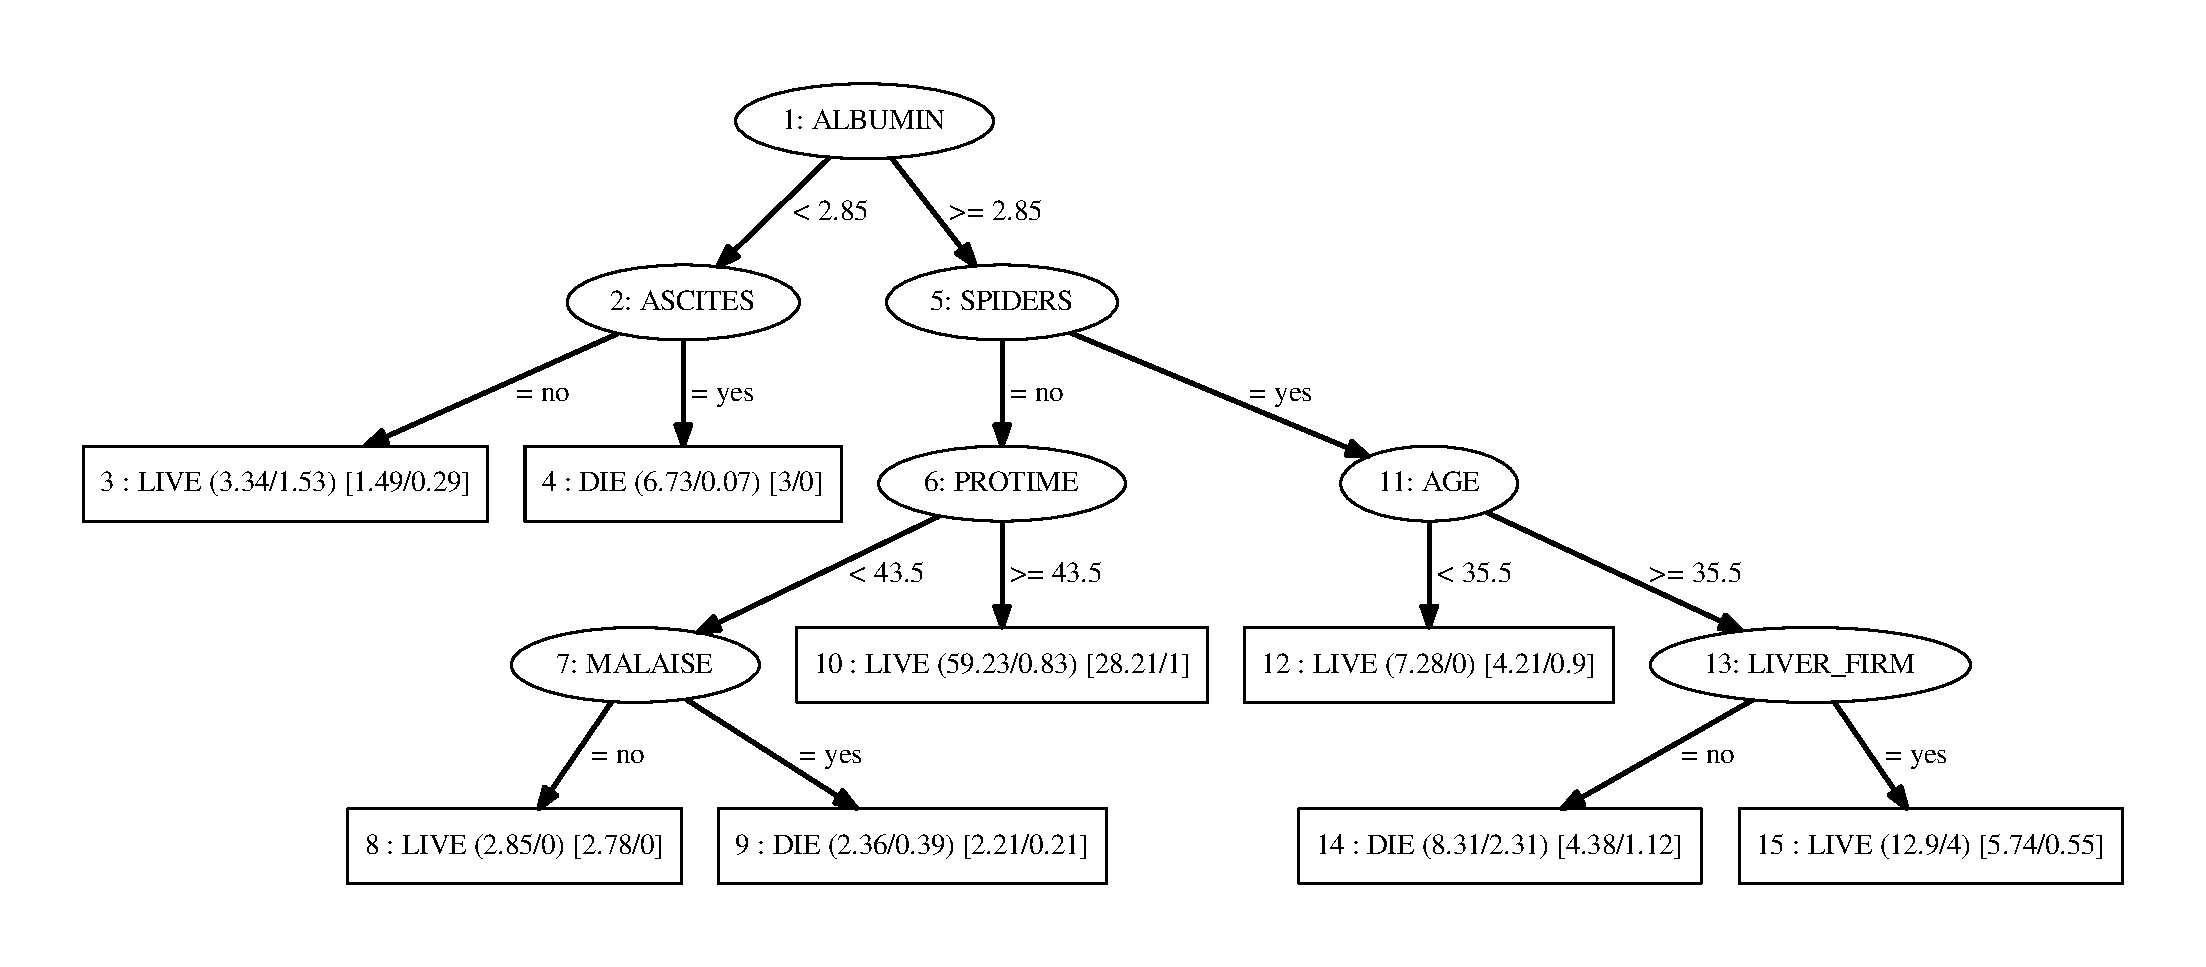
\includegraphics[width=1.55\textwidth]{results/reptree/hepatitis.pdf}}
	\caption{Modello di REPTree}
\end{figure}

\begin{mdframed}[frametitle=Esecuzione JRip]
	\footnotesize\verbatiminput{results/jrip/hepatitis.jrip}
\end{mdframed}


\noindent
\normalsize Regole:
\footnotesize\input{results/jrip/hepatitis.list.rules}

\pagebreak

\section{Risultati su \texttt{Vehicle Silhouettes}}

\normalsize L'esecuzione ha coinvolto 761 istanze di training e 85 istanze di testing ad ogni iterazione del CV.

\begin{mdframed}[frametitle=Esecuzione NaiveBayesSimple]
	\footnotesize\verbatiminput{results/nb/vehicle.nb}
\end{mdframed}


\scriptsize
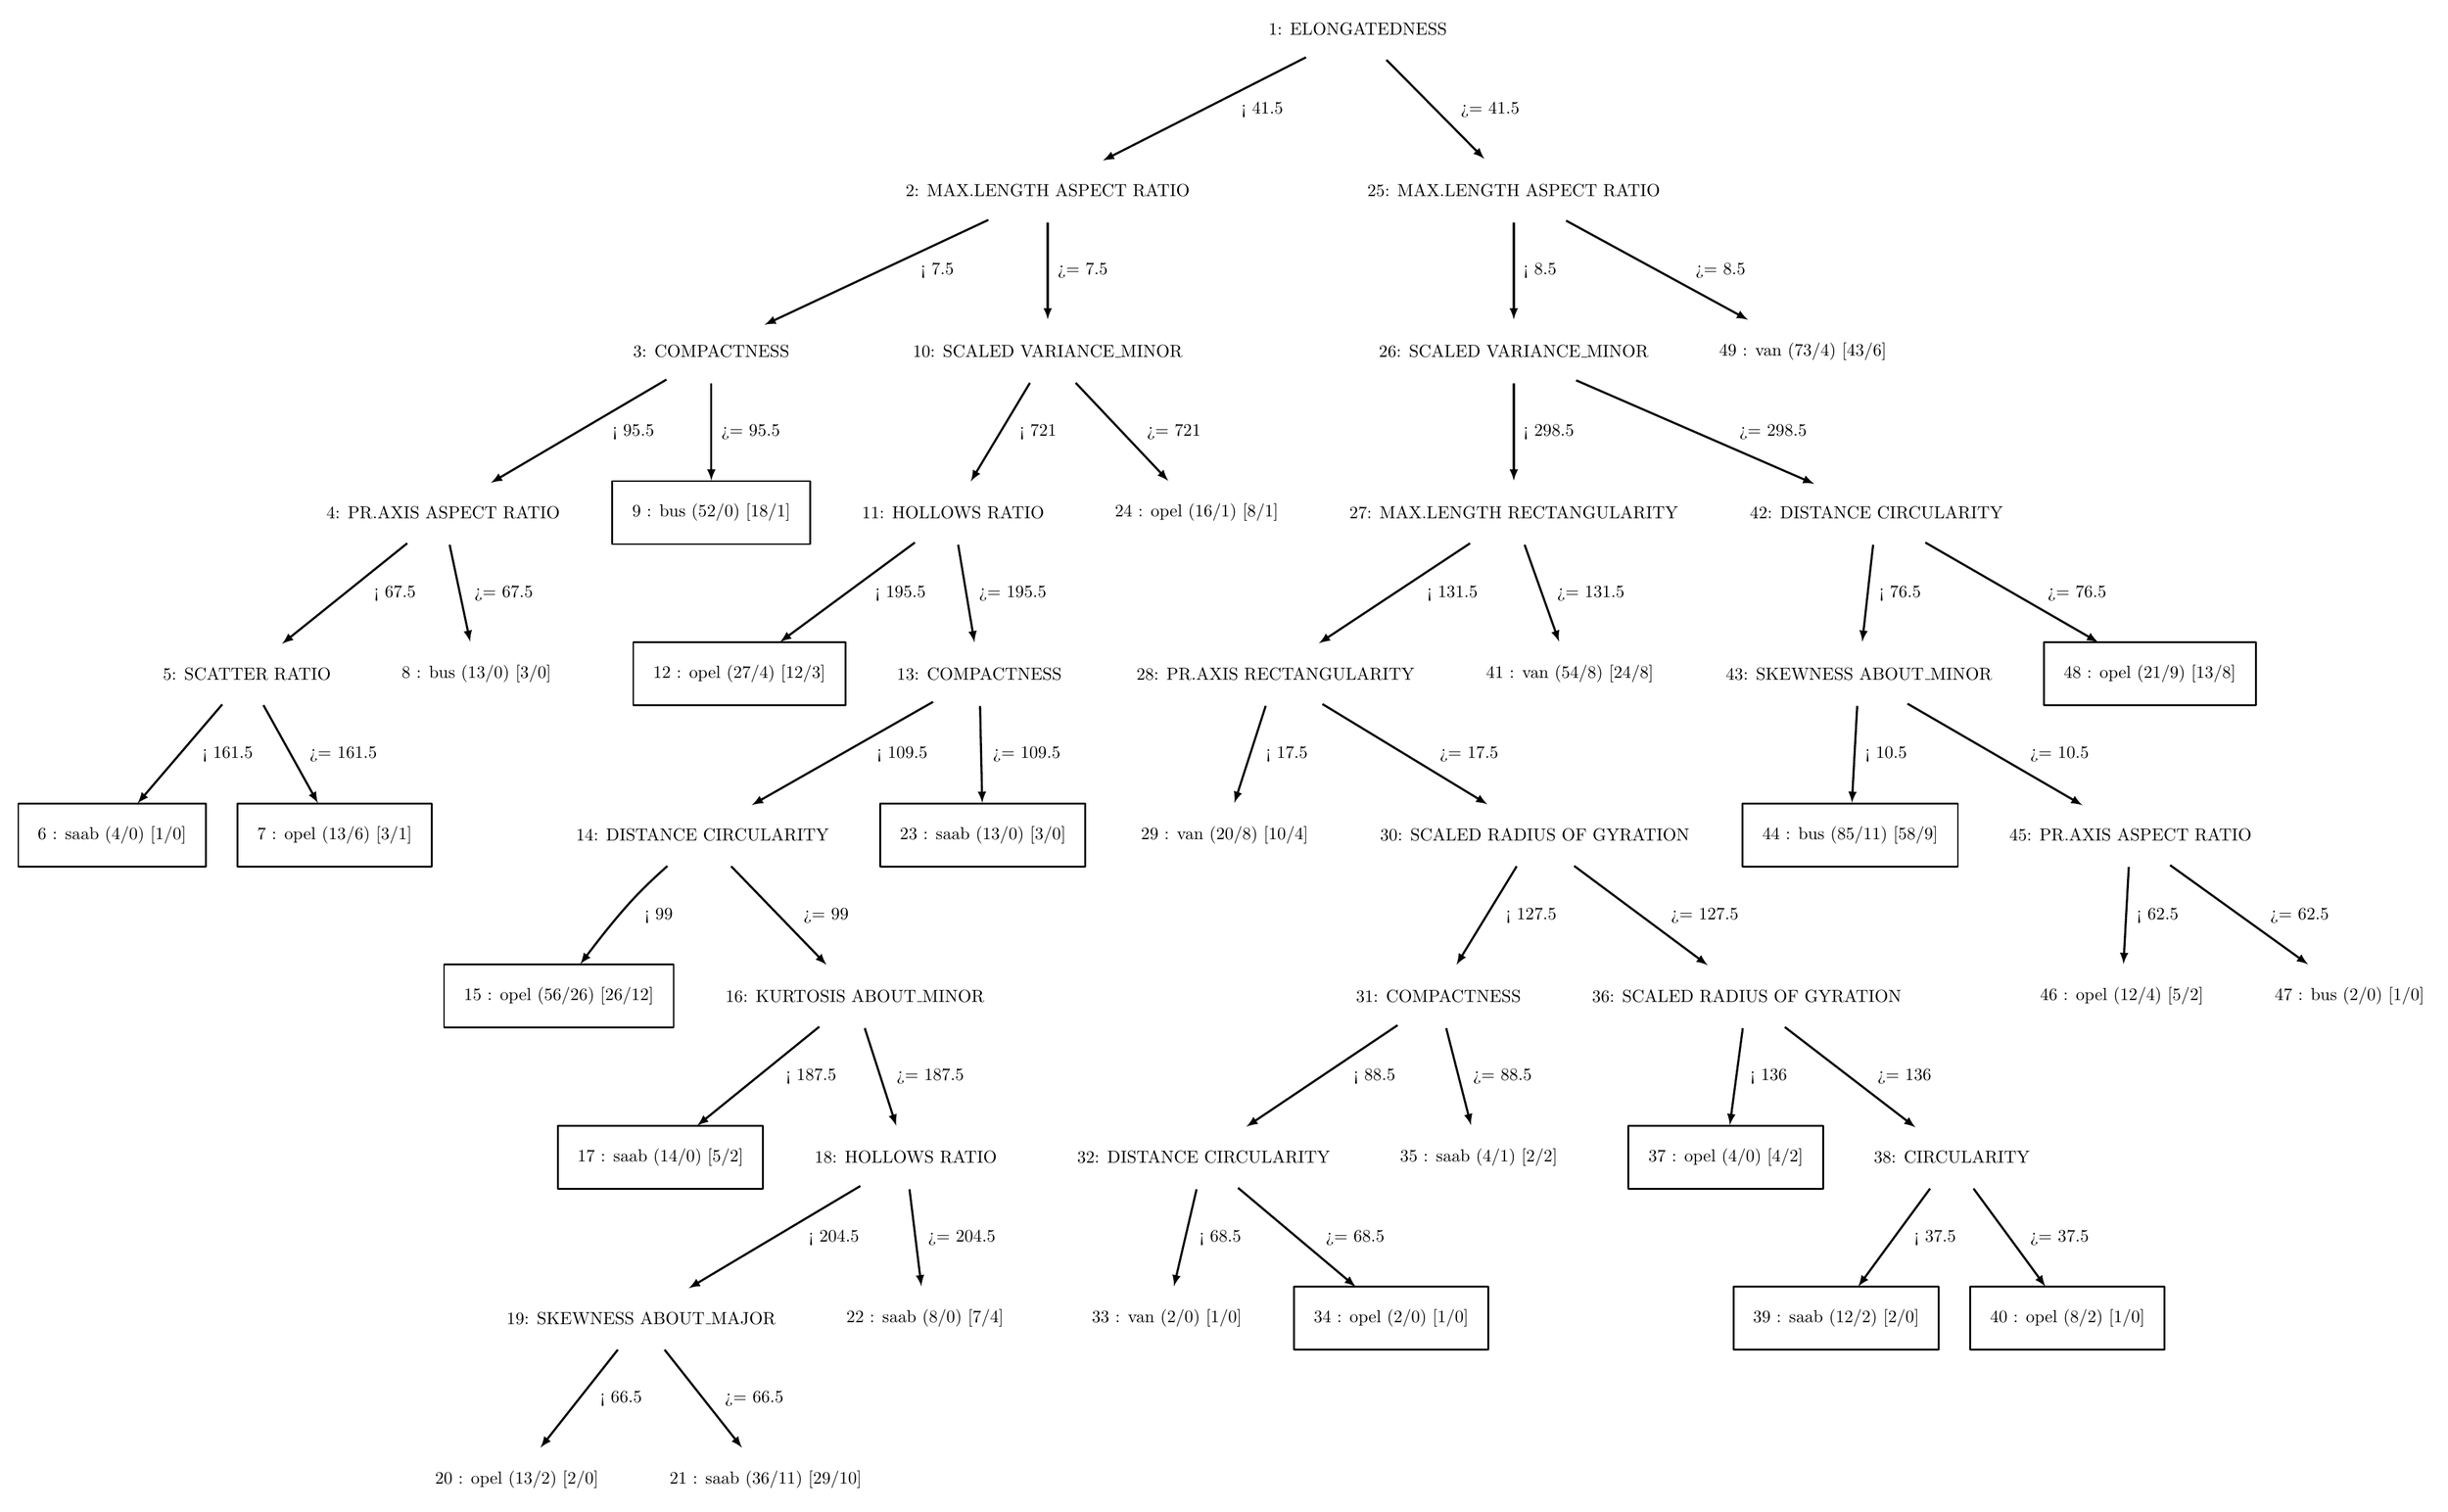
\begin{tikzpicture}[>=latex,line join=bevel,]
  \pgfsetlinewidth{1bp}
%%
\pgfsetcolor{black}
  % Edge: N4cdf35a9 -> N4c98385c
  \draw [->,very thick] (855.15bp,368.07bp) .. controls (847.01bp,354.75bp) and (835.53bp,335.95bp)  .. (820.8bp,311.85bp);
  \definecolor{strokecol}{rgb}{0.0,0.0,0.0};
  \pgfsetstrokecolor{strokecol}
  \draw (863.5bp,340.0bp) node { < 127.5};
  % Edge: N442d9b6e -> N15615099
  \draw [->,very thick] (1228.1bp,368.7bp) .. controls (1247.8bp,354.57bp) and (1276.4bp,333.96bp)  .. (1306.8bp,312.1bp);
  \draw (1302.0bp,340.0bp) node { >= 62.5};
  % Edge: N20fa23c1 -> N3581c5f3
  \draw [->,very thick] (221.96bp,552.49bp) .. controls (204.16bp,538.19bp) and (178.26bp,517.38bp)  .. (150.54bp,495.1bp);
  \draw (215.0bp,524.0bp) node { < 67.5};
  % Edge: N2b05039f -> N61e717c2
  \draw [->,very thick] (457.14bp,276.49bp) .. controls (439.84bp,262.46bp) and (414.79bp,242.15bp)  .. (387.48bp,220.01bp);
  \draw (452.5bp,248.0bp) node { < 187.5};
  % Edge: N484b61fc -> N45fe3ee3
  \draw [->,very thick] (711.91bp,459.65bp) .. controls (707.74bp,446.7bp) and (701.96bp,428.76bp)  .. (694.07bp,404.3bp);
  \draw (724.0bp,432.0bp) node { < 17.5};
  % Edge: N1a93a7ca -> N3d82c5f3
  \draw [->,very thick] (370.43bp,368.2bp) .. controls (364.15bp,362.63bp) and (357.34bp,356.25bp)  .. (351.5bp,350.0bp) .. controls (342.86bp,340.75bp) and (334.11bp,329.9bp)  .. (320.75bp,312.23bp);
  \draw (365.5bp,340.0bp) node { < 99};
  % Edge: N58d25a40 -> N1b701da1
  \draw [->,very thick] (1058.6bp,551.65bp) .. controls (1057.1bp,538.82bp) and (1055.2bp,521.11bp)  .. (1052.4bp,496.3bp);
  \draw (1074.0bp,524.0bp) node { < 76.5};
  % Edge: N4cdf35a9 -> N73a8dfcc
  \draw [->,very thick] (887.98bp,368.28bp) .. controls (907.16bp,354.01bp) and (934.93bp,333.36bp)  .. (964.14bp,311.63bp);
  \draw (962.5bp,340.0bp) node { >= 127.5};
  % Edge: N4dcbadb4 -> N17d10166
  \draw [->,very thick] (368.85bp,92.072bp) .. controls (379.5bp,78.581bp) and (394.56bp,59.486bp)  .. (412.96bp,36.158bp);
  \draw (420.0bp,64.0bp) node { >= 66.5};
  % Edge: N504bae78 -> N368102c8
  \draw [->,very thick] (883.38bp,736.7bp) .. controls (909.86bp,722.26bp) and (948.75bp,701.04bp)  .. (987.16bp,680.1bp);
  \draw (971.5bp,708.0bp) node { >= 8.5};
  % Edge: N3b764bce -> N759ebb3d
  \draw [->,very thick] (853.5bp,643.65bp) .. controls (853.5bp,630.82bp) and (853.5bp,613.11bp)  .. (853.5bp,588.3bp);
  \draw (873.5bp,616.0bp) node { < 298.5};
  % Edge: N73a8dfcc -> N7e774085
  \draw [->,very thick] (1008.2bp,276.28bp) .. controls (1026.9bp,261.9bp) and (1054.1bp,241.02bp)  .. (1082.7bp,219.02bp);
  \draw (1076.5bp,248.0bp) node { >= 136};
  % Edge: N3b764bce -> N58d25a40
  \draw [->,very thick] (889.08bp,645.53bp) .. controls (924.14bp,630.29bp) and (977.82bp,606.95bp)  .. (1025.0bp,586.42bp);
  \draw (1001.5bp,616.0bp) node { >= 298.5};
  % Edge: N593634ad -> N20fa23c1
  \draw [->,very thick] (369.89bp,645.94bp) .. controls (344.87bp,631.22bp) and (306.55bp,608.67bp)  .. (269.74bp,587.02bp);
  \draw (351.0bp,616.0bp) node { < 95.5};
  % Edge: N7506e922 -> N504bae78
  \draw [->,very thick] (780.82bp,828.49bp) .. controls (794.45bp,814.71bp) and (814.07bp,794.87bp)  .. (836.67bp,772.01bp);
  \draw (840.0bp,800.0bp) node { >= 41.5};
  % Edge: N20fa23c1 -> N73c6c3b2
  \draw [->,very thick] (246.16bp,551.65bp) .. controls (248.87bp,538.82bp) and (252.61bp,521.11bp)  .. (257.85bp,496.3bp);
  \draw (277.0bp,524.0bp) node { >= 67.5};
  % Edge: N7e0b37bc -> N6ae40994
  \draw [->,very thick] (536.39bp,551.65bp) .. controls (538.54bp,538.74bp) and (541.52bp,520.88bp)  .. (545.67bp,495.99bp);
  \draw (567.5bp,524.0bp) node { >= 195.5};
  % Edge: N593634ad -> N48533e64
  \draw [->,very thick] (395.5bp,643.65bp) .. controls (395.5bp,630.82bp) and (395.5bp,613.11bp)  .. (395.5bp,588.3bp);
  \draw (418.0bp,616.0bp) node { >= 95.5};
  % Edge: N73a8dfcc -> Nea30797
  \draw [->,very thick] (984.19bp,275.65bp) .. controls (982.48bp,262.82bp) and (980.11bp,245.11bp)  .. (976.81bp,220.3bp);
  \draw (999.0bp,248.0bp) node { < 136};
  % Edge: N442d9b6e -> Nee7d9f1
  \draw [->,very thick] (1204.5bp,367.65bp) .. controls (1203.8bp,354.82bp) and (1202.8bp,337.11bp)  .. (1201.5bp,312.3bp);
  \draw (1221.0bp,340.0bp) node { < 62.5};
  % Edge: N5fcfe4b2 -> N5eb5c224
  \draw [->,very thick] (696.13bp,184.49bp) .. controls (712.73bp,170.52bp) and (736.74bp,150.33bp)  .. (763.27bp,128.01bp);
  \draw (763.0bp,156.0bp) node { >= 68.5};
  % Edge: N2b05039f -> N66cd51c3
  \draw [->,very thick] (483.09bp,275.65bp) .. controls (487.29bp,262.62bp) and (493.12bp,244.53bp)  .. (501.02bp,219.99bp);
  \draw (520.5bp,248.0bp) node { >= 187.5};
  % Edge: N7e774085 -> N3f8f9dd6
  \draw [->,very thick] (1091.1bp,184.07bp) .. controls (1081.3bp,170.71bp) and (1067.4bp,151.84bp)  .. (1050.1bp,128.16bp);
  \draw (1094.0bp,156.0bp) node { < 37.5};
  % Edge: N66cd51c3 -> N1b9e1916
  \draw [->,very thick] (508.62bp,183.65bp) .. controls (510.19bp,170.82bp) and (512.35bp,153.11bp)  .. (515.39bp,128.3bp);
  \draw (538.5bp,156.0bp) node { >= 204.5};
  % Edge: N64a294a6 -> N4f8e5cde
  \draw [->,very thick] (603.49bp,644.07bp) .. controls (616.35bp,630.46bp) and (634.6bp,611.13bp)  .. (656.29bp,588.16bp);
  \draw (659.5bp,616.0bp) node { >= 721};
  % Edge: N4ee285c6 -> N593634ad
  \draw [->,very thick] (553.62bp,737.12bp) .. controls (520.55bp,721.62bp) and (470.26bp,698.04bp)  .. (425.88bp,677.24bp);
  \draw (524.5bp,708.0bp) node { < 7.5};
  % Edge: N484b61fc -> N4cdf35a9
  \draw [->,very thick] (744.3bp,460.7bp) .. controls (768.25bp,446.14bp) and (803.52bp,424.69bp)  .. (838.4bp,403.48bp);
  \draw (828.0bp,432.0bp) node { >= 17.5};
  % Edge: N3581c5f3 -> N6aa8ceb6
  \draw [->,very thick] (116.38bp,460.49bp) .. controls (104.69bp,446.84bp) and (87.923bp,427.23bp)  .. (68.057bp,404.01bp);
  \draw (119.5bp,432.0bp) node { < 161.5};
  % Edge: N7e774085 -> Naec6354
  \draw [->,very thick] (1115.9bp,184.07bp) .. controls (1125.7bp,170.71bp) and (1139.6bp,151.84bp)  .. (1156.9bp,128.16bp);
  \draw (1165.0bp,156.0bp) node { >= 37.5};
  % Edge: N58d25a40 -> N1edf1c96
  \draw [->,very thick] (1088.4bp,552.91bp) .. controls (1113.5bp,538.45bp) and (1150.5bp,517.08bp)  .. (1187.0bp,496.02bp);
  \draw (1175.0bp,524.0bp) node { >= 76.5};
  % Edge: N3581c5f3 -> N2530c12
  \draw [->,very thick] (139.9bp,460.07bp) .. controls (147.26bp,446.83bp) and (157.62bp,428.19bp)  .. (170.97bp,404.16bp);
  \draw (185.5bp,432.0bp) node { >= 161.5};
  % Edge: N64a294a6 -> N7e0b37bc
  \draw [->,very thick] (577.34bp,644.07bp) .. controls (569.35bp,630.75bp) and (558.07bp,611.95bp)  .. (543.61bp,587.85bp);
  \draw (582.0bp,616.0bp) node { < 721};
  % Edge: N4c98385c -> N53e25b76
  \draw [->,very thick] (814.93bp,275.65bp) .. controls (818.21bp,262.82bp) and (822.74bp,245.11bp)  .. (829.08bp,220.3bp);
  \draw (847.0bp,248.0bp) node { >= 88.5};
  % Edge: N759ebb3d -> N484b61fc
  \draw [->,very thick] (828.56bp,552.49bp) .. controls (806.7bp,538.03bp) and (774.77bp,516.9bp)  .. (742.29bp,495.4bp);
  \draw (818.5bp,524.0bp) node { < 131.5};
  % Edge: N5fcfe4b2 -> N6bf2d08e
  \draw [->,very thick] (672.45bp,183.65bp) .. controls (669.46bp,170.82bp) and (665.33bp,153.11bp)  .. (659.54bp,128.3bp);
  \draw (686.0bp,156.0bp) node { < 68.5};
  % Edge: N504bae78 -> N3b764bce
  \draw [->,very thick] (853.5bp,735.65bp) .. controls (853.5bp,722.82bp) and (853.5bp,705.11bp)  .. (853.5bp,680.3bp);
  \draw (868.5bp,708.0bp) node { < 8.5};
  % Edge: N4ee285c6 -> N64a294a6
  \draw [->,very thick] (587.5bp,735.65bp) .. controls (587.5bp,722.82bp) and (587.5bp,705.11bp)  .. (587.5bp,680.3bp);
  \draw (607.5bp,708.0bp) node { >= 7.5};
  % Edge: N6ae40994 -> N1a93a7ca
  \draw [->,very thick] (522.05bp,461.94bp) .. controls (496.21bp,447.22bp) and (456.64bp,424.67bp)  .. (418.63bp,403.02bp);
  \draw (504.5bp,432.0bp) node { < 109.5};
  % Edge: N1b701da1 -> N726f3b58
  \draw [->,very thick] (1049.5bp,459.65bp) .. controls (1048.8bp,446.82bp) and (1047.8bp,429.11bp)  .. (1046.5bp,404.3bp);
  \draw (1066.0bp,432.0bp) node { < 10.5};
  % Edge: N4c98385c -> N5fcfe4b2
  \draw [->,very thick] (787.16bp,277.32bp) .. controls (765.65bp,262.88bp) and (733.52bp,241.3bp)  .. (700.93bp,219.41bp);
  \draw (774.0bp,248.0bp) node { < 88.5};
  % Edge: N4dcbadb4 -> N4e515669
  \draw [->,very thick] (342.15bp,92.072bp) .. controls (331.5bp,78.581bp) and (316.44bp,59.486bp)  .. (298.04bp,36.158bp);
  \draw (344.0bp,64.0bp) node { < 66.5};
  % Edge: N759ebb3d -> N1c655221
  \draw [->,very thick] (859.67bp,551.65bp) .. controls (864.27bp,538.7bp) and (870.65bp,520.76bp)  .. (879.35bp,496.3bp);
  \draw (897.5bp,524.0bp) node { >= 131.5};
  % Edge: N6ae40994 -> Nba8a1dc
  \draw [->,very thick] (548.89bp,459.65bp) .. controls (549.17bp,446.82bp) and (549.56bp,429.11bp)  .. (550.12bp,404.3bp);
  \draw (575.5bp,432.0bp) node { >= 109.5};
  % Edge: N66cd51c3 -> N4dcbadb4
  \draw [->,very thick] (480.54bp,185.53bp) .. controls (456.0bp,170.9bp) and (418.94bp,148.81bp)  .. (382.65bp,127.18bp);
  \draw (465.5bp,156.0bp) node { < 204.5};
  % Edge: N1b701da1 -> N442d9b6e
  \draw [->,very thick] (1078.2bp,460.91bp) .. controls (1103.7bp,446.13bp) and (1141.6bp,424.13bp)  .. (1178.0bp,402.95bp);
  \draw (1165.0bp,432.0bp) node { >= 10.5};
  % Edge: N7e0b37bc -> N3b95a09c
  \draw [->,very thick] (511.69bp,552.91bp) .. controls (492.57bp,538.8bp) and (464.54bp,518.13bp)  .. (434.78bp,496.18bp);
  \draw (503.5bp,524.0bp) node { < 195.5};
  % Edge: N7506e922 -> N4ee285c6
  \draw [->,very thick] (734.87bp,829.94bp) .. controls (705.67bp,815.09bp) and (660.82bp,792.28bp)  .. (619.01bp,771.02bp);
  \draw (710.0bp,800.0bp) node { < 41.5};
  % Edge: N1a93a7ca -> N2b05039f
  \draw [->,very thick] (406.86bp,368.07bp) .. controls (420.23bp,354.24bp) and (439.29bp,334.53bp)  .. (461.21bp,311.85bp);
  \draw (461.0bp,340.0bp) node { >= 99};
  % Node: N2b05039f
\begin{scope}
  \definecolor{strokecol}{rgb}{0.0,0.0,0.0};
  \pgfsetstrokecolor{strokecol}
  \draw (477.5bp,294.0bp) node {16: KURTOSIS ABOUT\_MINOR};
\end{scope}
  % Node: N1b701da1
\begin{scope}
  \definecolor{strokecol}{rgb}{0.0,0.0,0.0};
  \pgfsetstrokecolor{strokecol}
  \draw (1050.5bp,478.0bp) node {43: SKEWNESS ABOUT\_MINOR};
\end{scope}
  % Node: N4e515669
\begin{scope}
  \definecolor{strokecol}{rgb}{0.0,0.0,0.0};
  \pgfsetstrokecolor{strokecol}
  \draw (284.5bp,18.0bp) node {20 : opel (13/2) [2/0]};
\end{scope}
  % Node: N17d10166
\begin{scope}
  \definecolor{strokecol}{rgb}{0.0,0.0,0.0};
  \pgfsetstrokecolor{strokecol}
  \draw (426.5bp,18.0bp) node {21 : saab (36/11) [29/10]};
\end{scope}
  % Node: N6aa8ceb6
\begin{scope}
  \definecolor{strokecol}{rgb}{0.0,0.0,0.0};
  \pgfsetstrokecolor{strokecol}
  \draw (107.0bp,404.0bp) -- (0.0bp,404.0bp) -- (0.0bp,368.0bp) -- (107.0bp,368.0bp) -- cycle;
  \draw (53.5bp,386.0bp) node {6 : saab (4/0) [1/0]};
\end{scope}
  % Node: N1a93a7ca
\begin{scope}
  \definecolor{strokecol}{rgb}{0.0,0.0,0.0};
  \pgfsetstrokecolor{strokecol}
  \draw (390.5bp,386.0bp) node {14: DISTANCE CIRCULARITY};
\end{scope}
  % Node: N4ee285c6
\begin{scope}
  \definecolor{strokecol}{rgb}{0.0,0.0,0.0};
  \pgfsetstrokecolor{strokecol}
  \draw (587.5bp,754.0bp) node {2: MAX.LENGTH ASPECT RATIO};
\end{scope}
  % Node: N66cd51c3
\begin{scope}
  \definecolor{strokecol}{rgb}{0.0,0.0,0.0};
  \pgfsetstrokecolor{strokecol}
  \draw (506.5bp,202.0bp) node {18: HOLLOWS RATIO};
\end{scope}
  % Node: N5eb5c224
\begin{scope}
  \definecolor{strokecol}{rgb}{0.0,0.0,0.0};
  \pgfsetstrokecolor{strokecol}
  \draw (839.0bp,128.0bp) -- (728.0bp,128.0bp) -- (728.0bp,92.0bp) -- (839.0bp,92.0bp) -- cycle;
  \draw (783.5bp,110.0bp) node {34 : opel (2/0) [1/0]};
\end{scope}
  % Node: Nee7d9f1
\begin{scope}
  \definecolor{strokecol}{rgb}{0.0,0.0,0.0};
  \pgfsetstrokecolor{strokecol}
  \draw (1200.5bp,294.0bp) node {46 : opel (12/4) [5/2]};
\end{scope}
  % Node: N368102c8
\begin{scope}
  \definecolor{strokecol}{rgb}{0.0,0.0,0.0};
  \pgfsetstrokecolor{strokecol}
  \draw (1018.5bp,662.0bp) node {49 : van (73/4) [43/6]};
\end{scope}
  % Node: N1c655221
\begin{scope}
  \definecolor{strokecol}{rgb}{0.0,0.0,0.0};
  \pgfsetstrokecolor{strokecol}
  \draw (885.5bp,478.0bp) node {41 : van (54/8) [24/8]};
\end{scope}
  % Node: N7e0b37bc
\begin{scope}
  \definecolor{strokecol}{rgb}{0.0,0.0,0.0};
  \pgfsetstrokecolor{strokecol}
  \draw (533.5bp,570.0bp) node {11: HOLLOWS RATIO};
\end{scope}
  % Node: Naec6354
\begin{scope}
  \definecolor{strokecol}{rgb}{0.0,0.0,0.0};
  \pgfsetstrokecolor{strokecol}
  \draw (1225.0bp,128.0bp) -- (1114.0bp,128.0bp) -- (1114.0bp,92.0bp) -- (1225.0bp,92.0bp) -- cycle;
  \draw (1169.5bp,110.0bp) node {40 : opel (8/2) [1/0]};
\end{scope}
  % Node: N2530c12
\begin{scope}
  \definecolor{strokecol}{rgb}{0.0,0.0,0.0};
  \pgfsetstrokecolor{strokecol}
  \draw (236.0bp,404.0bp) -- (125.0bp,404.0bp) -- (125.0bp,368.0bp) -- (236.0bp,368.0bp) -- cycle;
  \draw (180.5bp,386.0bp) node {7 : opel (13/6) [3/1]};
\end{scope}
  % Node: N504bae78
\begin{scope}
  \definecolor{strokecol}{rgb}{0.0,0.0,0.0};
  \pgfsetstrokecolor{strokecol}
  \draw (853.5bp,754.0bp) node {25: MAX.LENGTH ASPECT RATIO};
\end{scope}
  % Node: N484b61fc
\begin{scope}
  \definecolor{strokecol}{rgb}{0.0,0.0,0.0};
  \pgfsetstrokecolor{strokecol}
  \draw (717.5bp,478.0bp) node {28: PR.AXIS RECTANGULARITY};
\end{scope}
  % Node: N1edf1c96
\begin{scope}
  \definecolor{strokecol}{rgb}{0.0,0.0,0.0};
  \pgfsetstrokecolor{strokecol}
  \draw (1277.0bp,496.0bp) -- (1156.0bp,496.0bp) -- (1156.0bp,460.0bp) -- (1277.0bp,460.0bp) -- cycle;
  \draw (1216.5bp,478.0bp) node {48 : opel (21/9) [13/8]};
\end{scope}
  % Node: N4c98385c
\begin{scope}
  \definecolor{strokecol}{rgb}{0.0,0.0,0.0};
  \pgfsetstrokecolor{strokecol}
  \draw (810.5bp,294.0bp) node {31: COMPACTNESS};
\end{scope}
  % Node: N45fe3ee3
\begin{scope}
  \definecolor{strokecol}{rgb}{0.0,0.0,0.0};
  \pgfsetstrokecolor{strokecol}
  \draw (688.5bp,386.0bp) node {29 : van (20/8) [10/4]};
\end{scope}
  % Node: N726f3b58
\begin{scope}
  \definecolor{strokecol}{rgb}{0.0,0.0,0.0};
  \pgfsetstrokecolor{strokecol}
  \draw (1107.0bp,404.0bp) -- (984.0bp,404.0bp) -- (984.0bp,368.0bp) -- (1107.0bp,368.0bp) -- cycle;
  \draw (1045.5bp,386.0bp) node {44 : bus (85/11) [58/9]};
\end{scope}
  % Node: N4cdf35a9
\begin{scope}
  \definecolor{strokecol}{rgb}{0.0,0.0,0.0};
  \pgfsetstrokecolor{strokecol}
  \draw (865.5bp,386.0bp) node {30: SCALED RADIUS OF GYRATION};
\end{scope}
  % Node: N5fcfe4b2
\begin{scope}
  \definecolor{strokecol}{rgb}{0.0,0.0,0.0};
  \pgfsetstrokecolor{strokecol}
  \draw (676.5bp,202.0bp) node {32: DISTANCE CIRCULARITY};
\end{scope}
  % Node: N15615099
\begin{scope}
  \definecolor{strokecol}{rgb}{0.0,0.0,0.0};
  \pgfsetstrokecolor{strokecol}
  \draw (1330.5bp,294.0bp) node {47 : bus (2/0) [1/0]};
\end{scope}
  % Node: N442d9b6e
\begin{scope}
  \definecolor{strokecol}{rgb}{0.0,0.0,0.0};
  \pgfsetstrokecolor{strokecol}
  \draw (1205.5bp,386.0bp) node {45: PR.AXIS ASPECT RATIO};
\end{scope}
  % Node: N6bf2d08e
\begin{scope}
  \definecolor{strokecol}{rgb}{0.0,0.0,0.0};
  \pgfsetstrokecolor{strokecol}
  \draw (655.5bp,110.0bp) node {33 : van (2/0) [1/0]};
\end{scope}
  % Node: N3b764bce
\begin{scope}
  \definecolor{strokecol}{rgb}{0.0,0.0,0.0};
  \pgfsetstrokecolor{strokecol}
  \draw (853.5bp,662.0bp) node {26: SCALED VARIANCE\_MINOR};
\end{scope}
  % Node: N64a294a6
\begin{scope}
  \definecolor{strokecol}{rgb}{0.0,0.0,0.0};
  \pgfsetstrokecolor{strokecol}
  \draw (587.5bp,662.0bp) node {10: SCALED VARIANCE\_MINOR};
\end{scope}
  % Node: N3581c5f3
\begin{scope}
  \definecolor{strokecol}{rgb}{0.0,0.0,0.0};
  \pgfsetstrokecolor{strokecol}
  \draw (130.5bp,478.0bp) node {5: SCATTER RATIO};
\end{scope}
  % Node: Nba8a1dc
\begin{scope}
  \definecolor{strokecol}{rgb}{0.0,0.0,0.0};
  \pgfsetstrokecolor{strokecol}
  \draw (609.0bp,404.0bp) -- (492.0bp,404.0bp) -- (492.0bp,368.0bp) -- (609.0bp,368.0bp) -- cycle;
  \draw (550.5bp,386.0bp) node {23 : saab (13/0) [3/0]};
\end{scope}
  % Node: N58d25a40
\begin{scope}
  \definecolor{strokecol}{rgb}{0.0,0.0,0.0};
  \pgfsetstrokecolor{strokecol}
  \draw (1060.5bp,570.0bp) node {42: DISTANCE CIRCULARITY};
\end{scope}
  % Node: N48533e64
\begin{scope}
  \definecolor{strokecol}{rgb}{0.0,0.0,0.0};
  \pgfsetstrokecolor{strokecol}
  \draw (452.0bp,588.0bp) -- (339.0bp,588.0bp) -- (339.0bp,552.0bp) -- (452.0bp,552.0bp) -- cycle;
  \draw (395.5bp,570.0bp) node {9 : bus (52/0) [18/1]};
\end{scope}
  % Node: N759ebb3d
\begin{scope}
  \definecolor{strokecol}{rgb}{0.0,0.0,0.0};
  \pgfsetstrokecolor{strokecol}
  \draw (853.5bp,570.0bp) node {27: MAX.LENGTH RECTANGULARITY};
\end{scope}
  % Node: N1b9e1916
\begin{scope}
  \definecolor{strokecol}{rgb}{0.0,0.0,0.0};
  \pgfsetstrokecolor{strokecol}
  \draw (517.5bp,110.0bp) node {22 : saab (8/0) [7/4]};
\end{scope}
  % Node: N4f8e5cde
\begin{scope}
  \definecolor{strokecol}{rgb}{0.0,0.0,0.0};
  \pgfsetstrokecolor{strokecol}
  \draw (672.5bp,570.0bp) node {24 : opel (16/1) [8/1]};
\end{scope}
  % Node: N20fa23c1
\begin{scope}
  \definecolor{strokecol}{rgb}{0.0,0.0,0.0};
  \pgfsetstrokecolor{strokecol}
  \draw (242.5bp,570.0bp) node {4: PR.AXIS ASPECT RATIO};
\end{scope}
  % Node: N73c6c3b2
\begin{scope}
  \definecolor{strokecol}{rgb}{0.0,0.0,0.0};
  \pgfsetstrokecolor{strokecol}
  \draw (261.5bp,478.0bp) node {8 : bus (13/0) [3/0]};
\end{scope}
  % Node: N73a8dfcc
\begin{scope}
  \definecolor{strokecol}{rgb}{0.0,0.0,0.0};
  \pgfsetstrokecolor{strokecol}
  \draw (986.5bp,294.0bp) node {36: SCALED RADIUS OF GYRATION};
\end{scope}
  % Node: N4dcbadb4
\begin{scope}
  \definecolor{strokecol}{rgb}{0.0,0.0,0.0};
  \pgfsetstrokecolor{strokecol}
  \draw (355.5bp,110.0bp) node {19: SKEWNESS ABOUT\_MAJOR};
\end{scope}
  % Node: N6ae40994
\begin{scope}
  \definecolor{strokecol}{rgb}{0.0,0.0,0.0};
  \pgfsetstrokecolor{strokecol}
  \draw (548.5bp,478.0bp) node {13: COMPACTNESS};
\end{scope}
  % Node: N3f8f9dd6
\begin{scope}
  \definecolor{strokecol}{rgb}{0.0,0.0,0.0};
  \pgfsetstrokecolor{strokecol}
  \draw (1096.0bp,128.0bp) -- (979.0bp,128.0bp) -- (979.0bp,92.0bp) -- (1096.0bp,92.0bp) -- cycle;
  \draw (1037.5bp,110.0bp) node {39 : saab (12/2) [2/0]};
\end{scope}
  % Node: N7e774085
\begin{scope}
  \definecolor{strokecol}{rgb}{0.0,0.0,0.0};
  \pgfsetstrokecolor{strokecol}
  \draw (1103.5bp,202.0bp) node {38: CIRCULARITY};
\end{scope}
  % Node: N61e717c2
\begin{scope}
  \definecolor{strokecol}{rgb}{0.0,0.0,0.0};
  \pgfsetstrokecolor{strokecol}
  \draw (425.0bp,220.0bp) -- (308.0bp,220.0bp) -- (308.0bp,184.0bp) -- (425.0bp,184.0bp) -- cycle;
  \draw (366.5bp,202.0bp) node {17 : saab (14/0) [5/2]};
\end{scope}
  % Node: N53e25b76
\begin{scope}
  \definecolor{strokecol}{rgb}{0.0,0.0,0.0};
  \pgfsetstrokecolor{strokecol}
  \draw (833.5bp,202.0bp) node {35 : saab (4/1) [2/2]};
\end{scope}
  % Node: N7506e922
\begin{scope}
  \definecolor{strokecol}{rgb}{0.0,0.0,0.0};
  \pgfsetstrokecolor{strokecol}
  \draw (764.5bp,846.0bp) node {1: ELONGATEDNESS};
\end{scope}
  % Node: N593634ad
\begin{scope}
  \definecolor{strokecol}{rgb}{0.0,0.0,0.0};
  \pgfsetstrokecolor{strokecol}
  \draw (395.5bp,662.0bp) node {3: COMPACTNESS};
\end{scope}
  % Node: N3b95a09c
\begin{scope}
  \definecolor{strokecol}{rgb}{0.0,0.0,0.0};
  \pgfsetstrokecolor{strokecol}
  \draw (472.0bp,496.0bp) -- (351.0bp,496.0bp) -- (351.0bp,460.0bp) -- (472.0bp,460.0bp) -- cycle;
  \draw (411.5bp,478.0bp) node {12 : opel (27/4) [12/3]};
\end{scope}
  % Node: Nea30797
\begin{scope}
  \definecolor{strokecol}{rgb}{0.0,0.0,0.0};
  \pgfsetstrokecolor{strokecol}
  \draw (1030.0bp,220.0bp) -- (919.0bp,220.0bp) -- (919.0bp,184.0bp) -- (1030.0bp,184.0bp) -- cycle;
  \draw (974.5bp,202.0bp) node {37 : opel (4/0) [4/2]};
\end{scope}
  % Node: N3d82c5f3
\begin{scope}
  \definecolor{strokecol}{rgb}{0.0,0.0,0.0};
  \pgfsetstrokecolor{strokecol}
  \draw (374.0bp,312.0bp) -- (243.0bp,312.0bp) -- (243.0bp,276.0bp) -- (374.0bp,276.0bp) -- cycle;
  \draw (308.5bp,294.0bp) node {15 : opel (56/26) [26/12]};
\end{scope}
%
\end{tikzpicture}



\begin{mdframed}[frametitle=Esecuzione REPTree]
	\scriptsize\verbatiminput{results/reptree/vehicle.reptree}
\end{mdframed}


\begin{figure}[htb]
	\makebox[\textwidth]{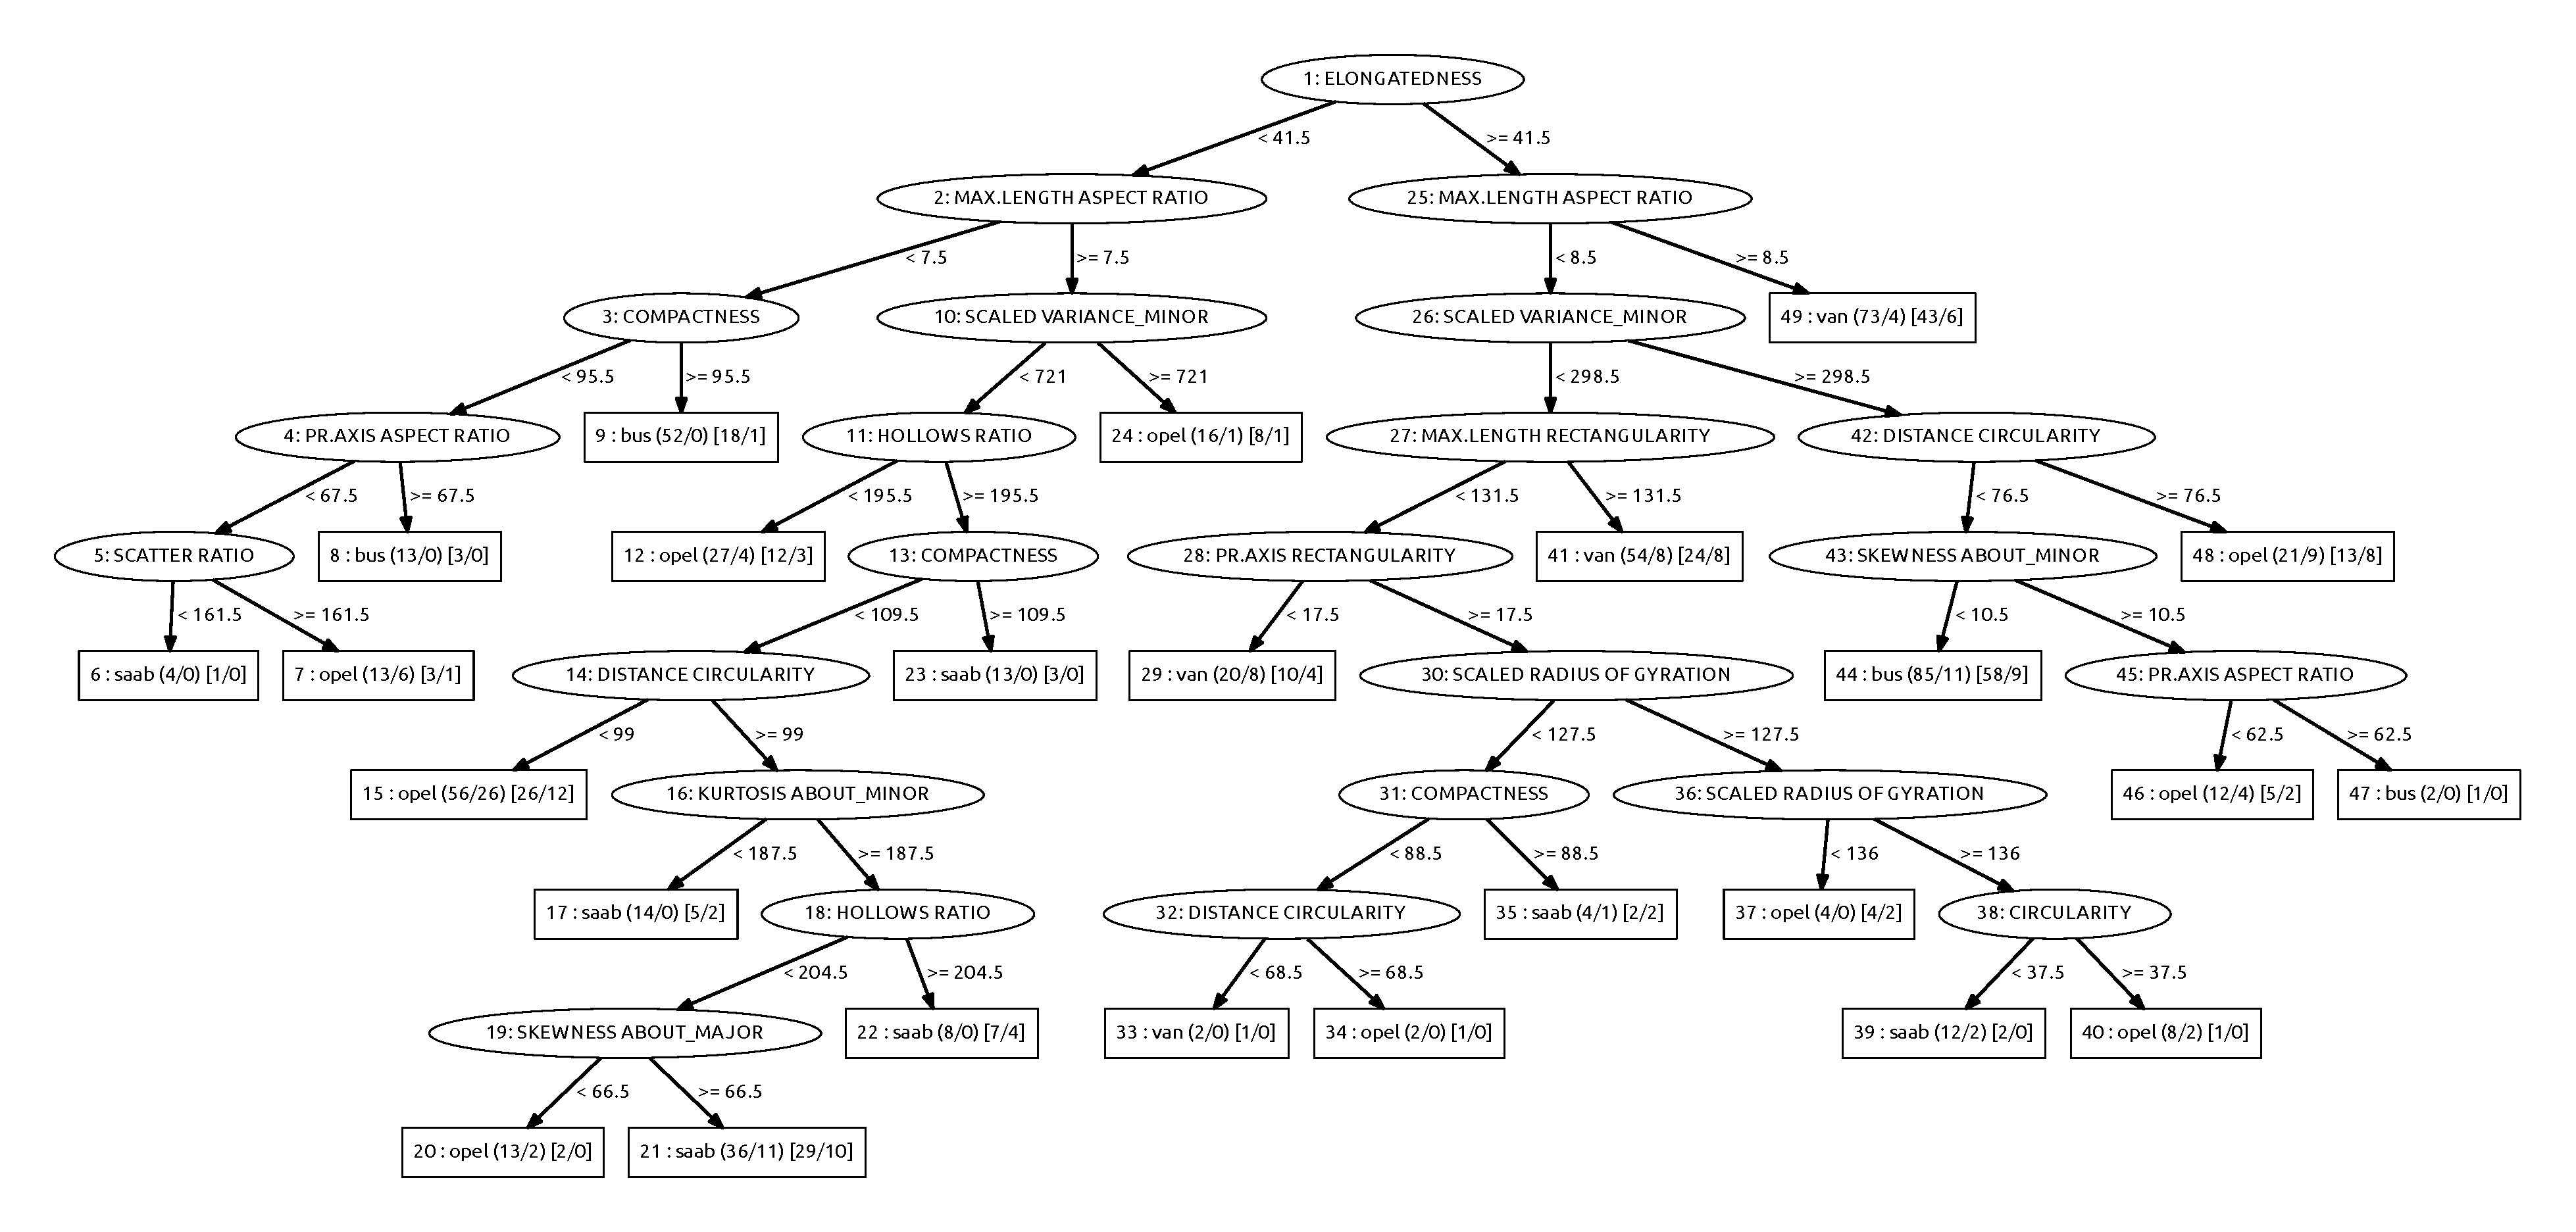
\includegraphics[width=1.55\textwidth]{results/reptree/vehicle.pdf}}
	\caption{Modello di REPTree}
\end{figure}

\begin{mdframed}[frametitle=Esecuzione JRip]
	\scriptsize\verbatiminput{results/jrip/vehicle.jrip}
\end{mdframed}


\noindent
\normalsize Regole:
\scriptsize\input{results/jrip/vehicle.list.rules}

\pagebreak

\section{Risultati su \texttt{Wisconsin Breast Cancer}}

\normalsize L'esecuzione ha coinvolto 629 istanze di training e 70 istanze di testing per ogni fold.


\begin{mdframed}[frametitle=Esecuzione NaiveBayesSimple]
	\footnotesize\verbatiminput{results/nb/wbc.nb}
\end{mdframed}


\footnotesize\input{results/nb/wbc.nbc}

\begin{mdframed}[frametitle=Esecuzione REPTree]
	\footnotesize\verbatiminput{results/reptree/wisconsin_breast_cancer.reptree}
\end{mdframed}


\begin{figure}[htb]
	\makebox[\textwidth]{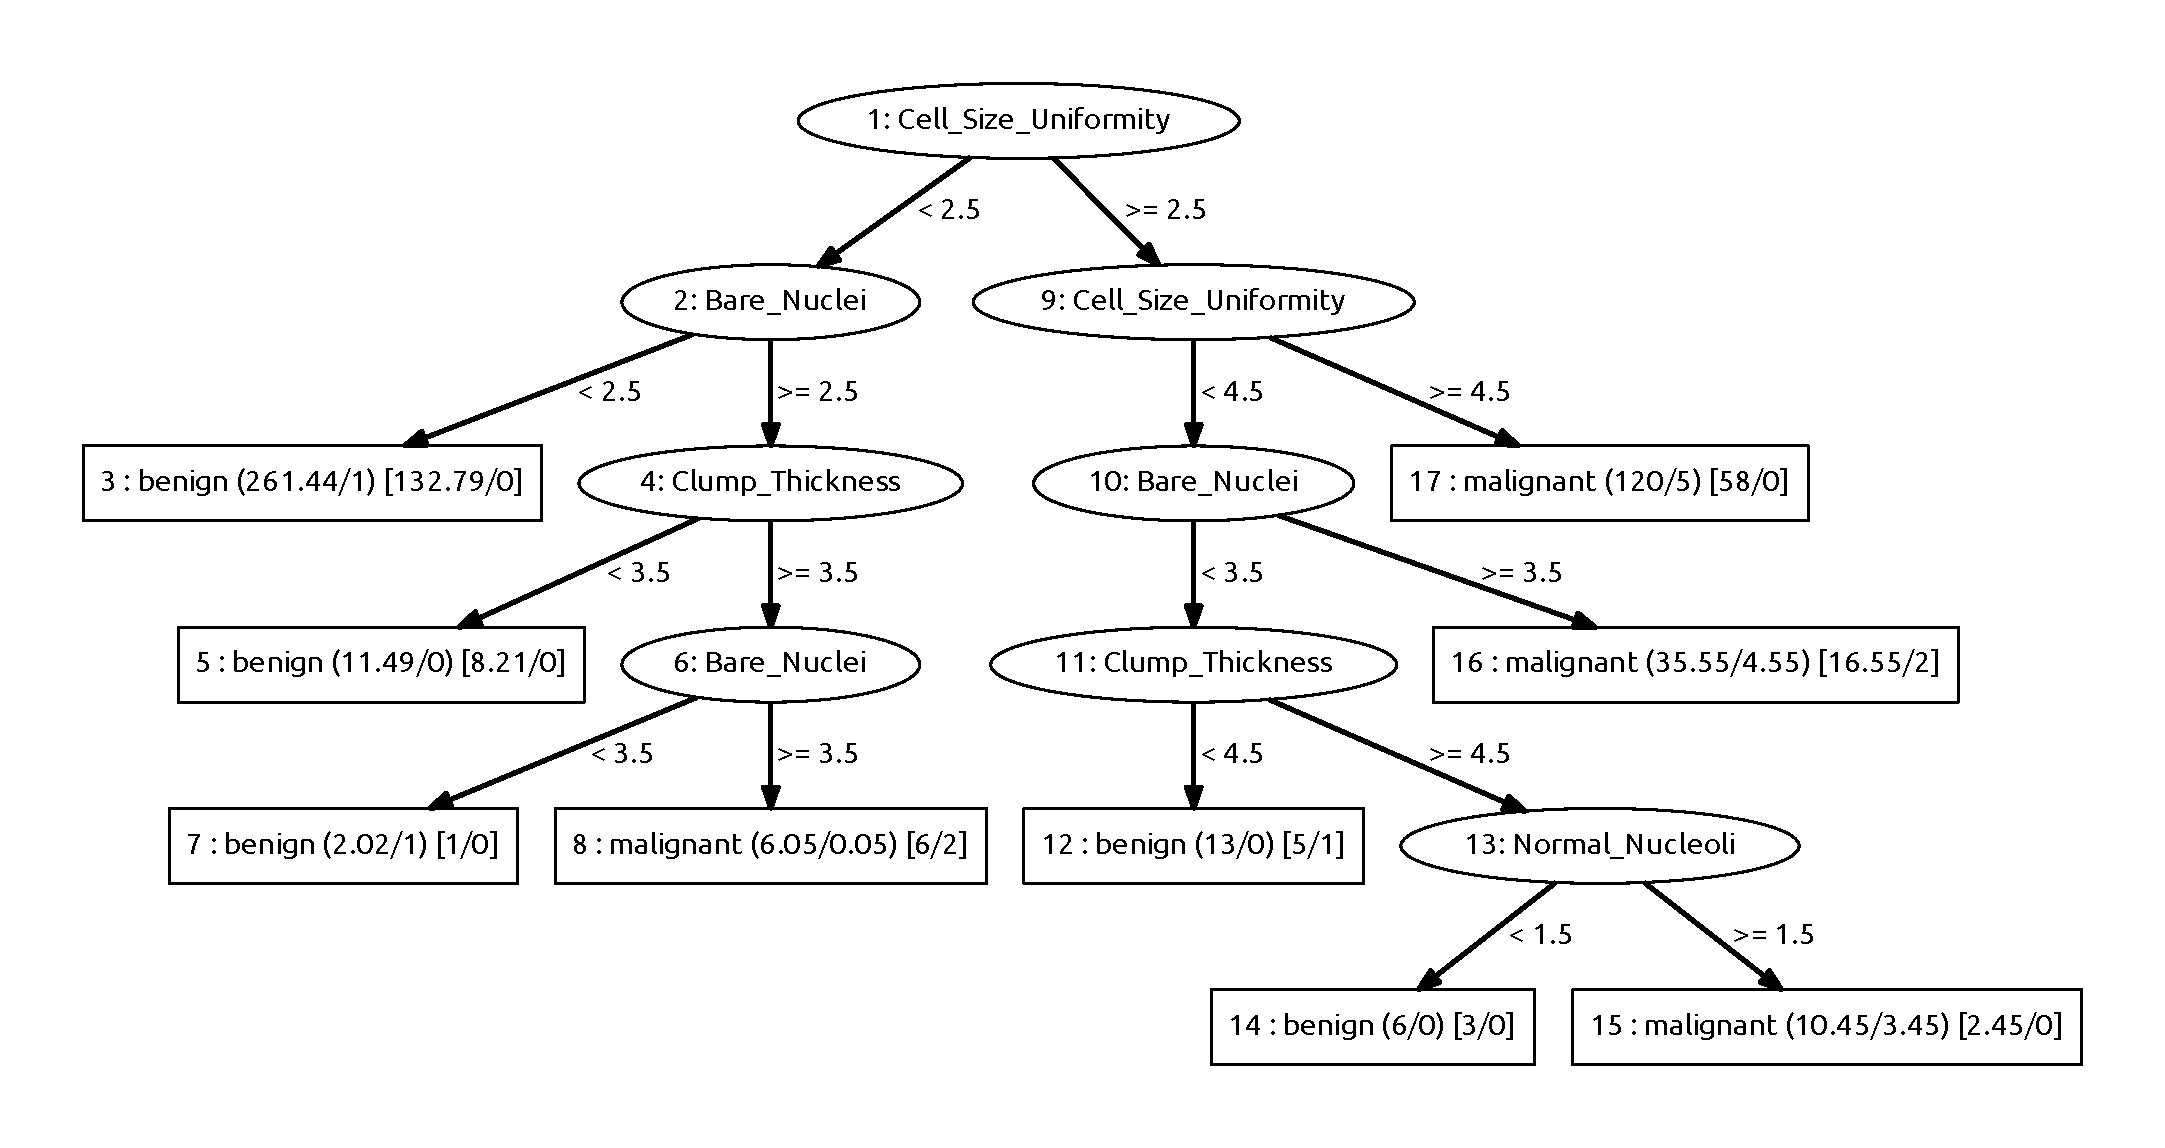
\includegraphics[width=1.55\textwidth]{results/reptree/wisconsin_breast_cancer.pdf}}
	\caption{Modello di REPTree}
\end{figure}

\begin{mdframed}[frametitle=Esecuzione JRip]
	\footnotesize\verbatiminput{results/jrip/wisconsin_breast_cancer.jrip}
\end{mdframed}


\noindent
\normalsize Regole:
\footnotesize\input{results/jrip/wisconsin_breast_cancer.list.rules}